\documentclass[../main.tex]{subfiles}
\begin{document}
\section{Neural Networks}
In this chapter we describe a class of learning methods that was developed separately in different fields-statistics and artificial intelligence—based on essentially identical models. The central idea is to extract linear combinations of the inputs as derived features, and then model the target as a nonlinear function of these features. The result is a powerful learning method, with widespread applications in many fields.

Neural network learning methods provide a robust approach to approximating real-valued, discrete-valued, and vector-valued target functions. For certain types of problems, such as learning to interpret complex real-world sensor data, artificial neural networks are among the most effective learning methods currently known. For example, the BACKPROPAGATION algorithm described in this chapter has proven surprisingly successful in many practical problems such as learning to recognize handwritten characters (LeCun et al. 1989), learning to recognize spoken words (Lang et al. 1990), and learning to recognize faces (Cottrell 1990). One survey of practical applications is provided by Rumelhart et al. (1994).

\subsection{Biological Motivation}
The study of artificial neural networks (ANNs) has been inspired in part by the observation that biological learning systems are built of very complex webs of interconnected neurons. In rough analogy, artificial neural networks are built out of a densely interconnected set of simple units, where each unit takes a number of real-valued inputs (possibly the outputs of other units) and produces a single real-valued output (which may become the input to many other units).

To develop a feel for this analogy, let us consider a few facts from neuro-biology. The human brain, for example, is estimated to contain a densely inter- connected network of approximately $10^{11}$ neurons, each connected, on average, to $10^4$ others. Neuron activity is typically excited or inhibited through connections to other neurons. The fastest neuron switching times are known to be on the order of $10^{-3}$ seconds--quite slow compared to computer switching speeds of $10^{-10}$ seconds. Yet humans are able to make surprisingly complex decisions, surprisingly quickly.

For example,it requires approximately $10^{-1}$ seconds to visually recognize your mother. Notice the sequence of neuron firings that can take place during this $10^{-1}$ second interval cannot possibly be longer than a few hundred steps, given the switching speed of single neurons. This observation has led many to speculate that the information-processing abilities of biological neural systems must follow from highly parallel processes operating on representations that are distributed over many neurons. One motivation for ANN systems is to capture this kind of highly parallel computation based on distributed representations. Most ANN software runs on sequential machines emulating distributed processes, although faster versions of the algorithms have also been implemented on highly parallel machines and on specialized hardware designed specifically for ANN applications.

While ANNs are loosely motivated by biological neural systems, there are many complexities to biological neural systems that are not modeled by ANNs, and many features of the ANNs we discuss here are known to be inconsistent with biological systems. For example, we consider here ANNs whose individual units output a single constant value, whereas biological neurons output a complex time series of spikes

\subsection{Appropriate problems for NN Learning}
ANN learning is well-suited to problems in which the training data corresponds to noisy, complex sensor data, such as inputs from cameras and microphones.
it is also applicable to problems for which more symbolic representations are often used, such as the decision tree learning tasks. ANN is appropriate for problems with the following characteristics:
\begin{itemize}
    \item\textit{Instances are represented by many attribute-value pairs}. The target function to be learned is defined over instances that can be described by a vector of predefined features, such as the pixel values. These input attributes may be highly correlated or independent of one another. Input values can be any real values.
    
    \item \textit{The target function output may be discrete-valued, real-valued, or a vector of several real- or discrete-valued attributes} 
    
    \item \textit{The training examples may contain errors}. ANN learning methods are quite robust to noise in the training data.
    
    \item \textit{Long training times are acceptable}. Network training algorithms typically require longer training times than, say, decision tree learning algorithms. Training times can range from a few seconds to many hours, depending on factors such as the number of weights in the network, the number of training examples considered, and the settings of various learning algorithm parameters.
    
    \item \textit{Fast evaluation of the learned target function may be required}. Although ANN learning times are relatively long, evaluating the learned network, in order to apply it to a subsequent instance, is typically very fast. 
    
    \item \textit{The ability of humans to understand the learned target function is not important}. The weights learned by neural networks are often difficult for humans to interpret. Learned neural networks are less easily communicated to humans than learned rules.
\end{itemize}

\subsection{Artificial Neuron: processing unit}
A neural network is composed of several neurons. Let's look at the single unit in detail.
\begin{itemize}
    \item Neuron, node or \textbf{unit}
    \item \emph{Inputs}: from extern source or other units, typically are real numbers
    \item \emph{Input Connections}: \textbf{weights \emph{w}}. Free parameters that can be modified by learning (synaptic strength).
\end{itemize}
\begin{figure}[H]
    \centering
    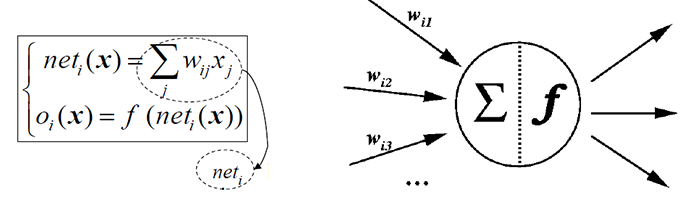
\includegraphics[scale = 0.6]{lectures/4_neural_networks/4_neuron.png}
    \caption{Processing unit}
    \label{fig:neuron}
\end{figure}
\begin{itemize}
    \item The weighted sum $net_i$ is called the \textbf{net input} to unit $i$
    \item Note that $w_{ij}$ refers to the weight of the unit $i$, in other words from unit $j$ to unit $i$ (not the other way around, this is a standard notation).
    \item The function $f$ is the unit's \textbf{activation function} (for example linear, LTU, ...).
    \item Output $o_i(\bold{x})$.
\end{itemize}

\subsection{Neuron: Three activation functions}
Changing the activation function we can have different neural networks.

\begin{itemize}
    \item \textbf{Linear activation function}
    $$ o = net = h(\mathbf{x}) = \sum_{i}^{} w_ix_i$$
    \begin{figure}[H]
        \centering
        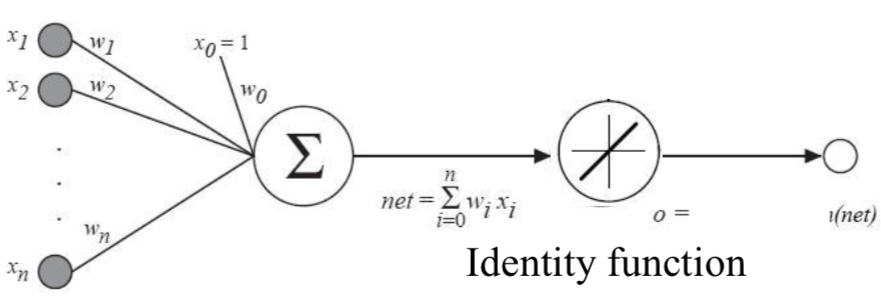
\includegraphics[scale = 0.3]{lectures/4_neural_networks/4_activation_function_linear_act.png}
    \end{figure}
    
    \item \textbf{Perceptron} (see LTU) Threshold activation function
    $$ o = \sigma(net) =  sign(net)$$
    \begin{figure}[H]
        \centering
        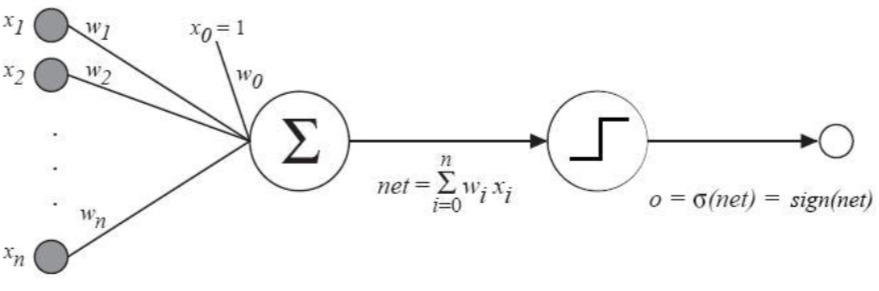
\includegraphics[scale = 0.3]{lectures/4_neural_networks/4_activation_function_ltu.png}
    \end{figure}
    
    \item \textbf{Logistic function}: sigmoid
    $$ o = \sigma(net) =  \frac{1}{1 - e^{-net}}$$
    \begin{figure}[H]
        \centering
        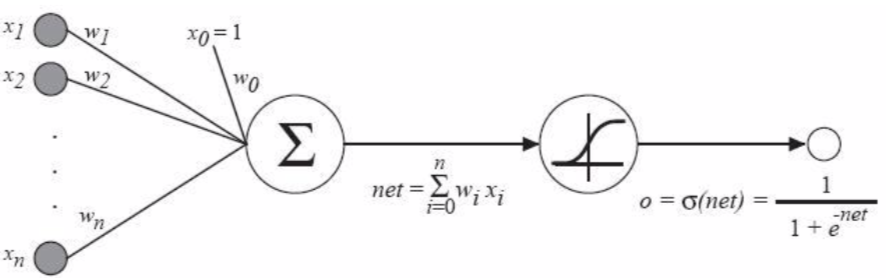
\includegraphics[scale = 0.3]{lectures/4_neural_networks/4_activation_function_sigmoid.png}
    \end{figure}
\end{itemize}


\subsection{Rosenblatt’s Perceptron}
In the formative years of neural networks (1943–1958), several researchers stand out for their pioneering contributions:
\begin{itemize}
    \item McCulloch and Pitts (1943) for introducing the idea of neural networks as computing machines.
    \item Hebb(1949) for postulating the first rule for self-organized learning.
    \item Rosenblatt (1958) for proposing the perceptron as the first model for learning with a teacher (i.e., supervised learning).
\end{itemize}

Rosenblatt’s perceptron is built around the McCulloch and Pitts model of a neuron (Biologically inspired model) and this is a model of historical importance for the ML, with different approaches since the early 60s.
This neural networks system si base on the unit called a \emph{perceptron} (Rosenblatt, 1958) illustrated in Figure~\ref{fig:perceptron}, it is suitable for automated learning (there is a learning algorithm) and it has well-defined computational properties (Convergence theorem).
\begin{figure}[H]
    \centering
    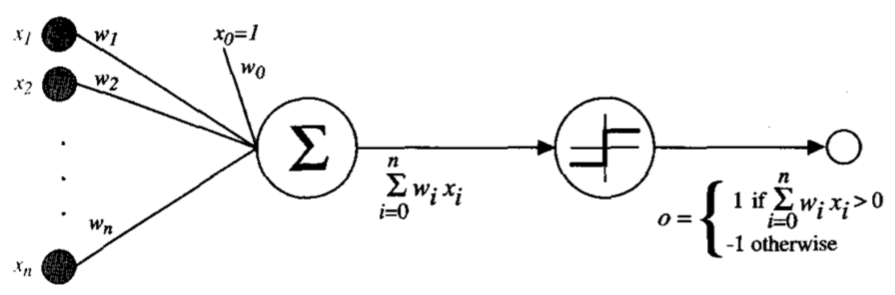
\includegraphics[scale = 0.35]{lectures/4_neural_networks/4_perceptron.png}
    \caption{Perceptron}
    \label{fig:perceptron}
\end{figure}
The \emph{perceptron} is the simplest form of a neural network used for the classifi- cation of patterns said to be linearly separable (i.e., patterns that lie on opposite sides of a hyperplane).

\noindent It takes a vector of real-valued inputs, calculates a linear combination of these inputs, then outputs a $1$ if the result is greater than some threshold and $-1$ otherwise. More precisely, given inputs $x_l$ through $x_n$, the output $o(x_1, . . . , x_n)$ computed by the perceptron is
\begin{figure}[H]
    \centering
    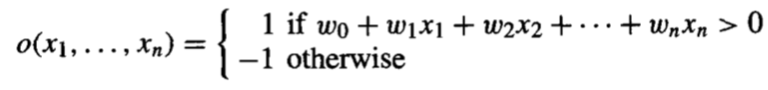
\includegraphics[scale = 0.35]{lectures/4_neural_networks/4_out_perc.png}
    \label{fig:out_perc}
\end{figure}
\noindent where each $w_i$ is a real-valued constant, or \textbf{weight}, that determines the contribution of input $x_i$ to the perceptron output (for brevity $o(\bold{x})=sgn(\bold{wx})$). Notice the quantity ($-w_O$) is a threshold that the weighted combination of inputs $w_lx_l + . . . + w_nx_n$ must surpass in order for the perceptron to output a $1$.\\

\subsubsection{Representational Power of Perceptron}
We can view the perceptron as representing a hyperplane decision surface in the $n$-dimensional space of instances (i.e., points). The perceptron outputs a $1$ for instances lying on one side of the hyperplane and outputs a $-1$ for instances lying on the other side, as illustrated in Figure~\ref{fig:4_percp_linear_sep_and_no}.

\begin{figure}
    \centering
    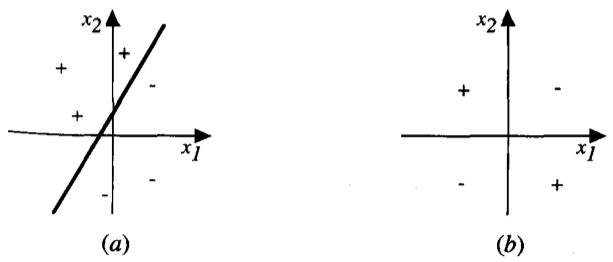
\includegraphics[scale = 0.4]{lectures/4_neural_networks/4_percp_linear_sep_and_no.png}
    \caption{The decision surface represented by a two-input perceptron. (a) A set of training examples and the decision surface of a perceptron that classifies them correctly. (b) A set of training examples that is not linearly separable (i.e., that cannot be correctly classified by any straight line). x l and x2 are the Perceptron inputs. Positive examples are indicated by "+", negative by "-".}
    \label{fig:4_percp_linear_sep_and_no}
\end{figure}

The equation for this decision hyperplane is $wx = 0$. Of course, some sets of positive and negative examples cannot be separated by any hyperplane. Those that can be separated are called \textit{linearly separable} sets of examples.\\

A single perceptron can be used to represent many boolean functions. For example, if we assume boolean values of $1$ (true) and $-1$ (false), then one way to use a two-input perceptron to implement the AND function is to set the weights $w_0 = -8$, and $w_l = w_2 = .5$. This perceptron can be made to represent the OR function instead by altering the threshold to $w_0 = -.3$, see Figure~\ref{fig:4_boolean_functions}.

A single perceptron can be used to represent many boolean functions (for example AND, OR, NAND and NOR boolean functions). The ability of perceptrons to represent AND, OR, NAND, and NOR is important because every boolean function can be represented by some network of interconnected units based on these primitives. In fact, every boolean function can be represented by some network of perceptrons only two levels deep, in which the inputs are fed to multiple units, and the outputs of these units are then input to a second, final stage. One way is to represent the boolean function in disjunctive normal form (i.e., as the disjunction (OR) of a set of conjunctions (ANDs) of the inputs and their negations). Note that the input to an AND perceptron can be negated simply by changing the sign of the corresponding input weight. Because networks of threshold units can represent a rich variety of functions and because single units alone cannot, we will generally be interested in learning multilayer networks of threshold units
\begin{figure}[H]
    \centering
    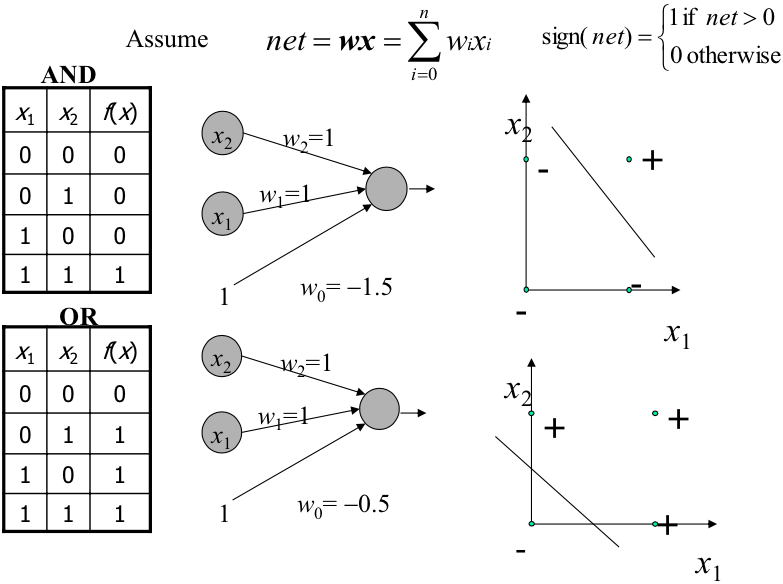
\includegraphics[scale = 0.3]{lectures/4_neural_networks/4_boolean_functions.png}
    \caption{AND, OR Boolean functions}
    \label{fig:4_boolean_functions}
\end{figure}
\noindent Unfortunately, however, some boolean functions cannot be represented by a single perceptron, such as the XOR function.

Unfortunately, however, some boolean functions cannot be represented by a single perceptron, such as the XOR function whose value is 1 if and only if $x_l \neq x_2$. Note the set is linearly nonseparable.
\begin{figure}[H]
    \centering
    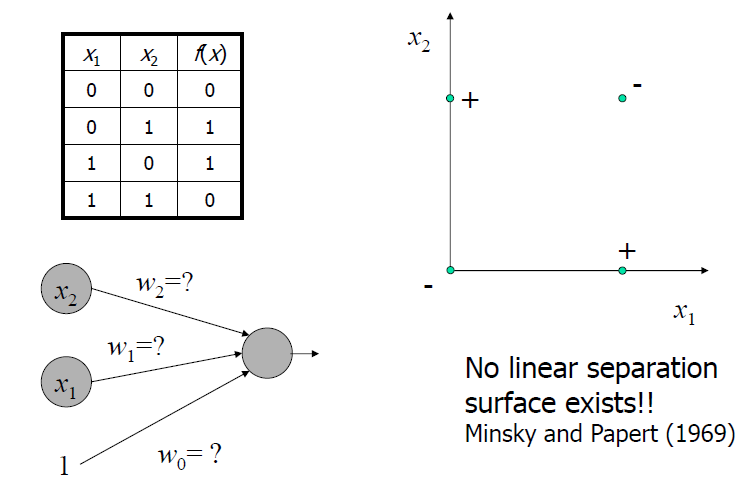
\includegraphics[scale = 0.6]{lectures/4_neural_networks/4_onelayer_xor.png}
    \label{fig:onelayer_xor}
    \caption{Exclusive OR (XOR)}
\end{figure}
\noindent To represent the XOR we can use a \emph{two layers network}, where $h_1,\, h_2$ are \textbf{hidden layers}.
\begin{figure}[H]
    \centering
    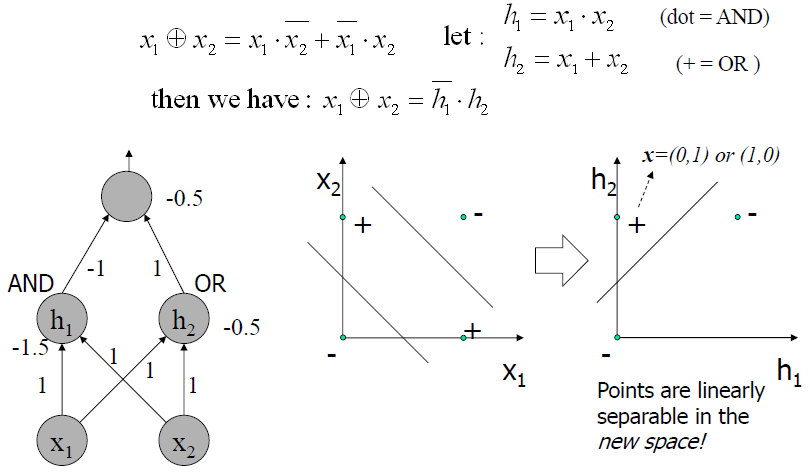
\includegraphics[scale = 0.6]{lectures/4_neural_networks/4_xor_two.png}
    \label{fig:xor_two}
    \caption{XOR by a Two Layers Network}
\end{figure}

\subsection{Learning for one unit model}
Two kinds of method for learning
\begin{itemize}
    \item \textbf{ADALINE (Adaptive Linear Neuron)} is an early single-layer artificial neural network (Widrow, Hoff). It is based on the McCulloch–Pitts neuron. It consists of a weight, a bias and a summation function. See Figure~\ref{fig:4_Adaline_flow_chart}.
    
    \begin{figure}
        \centering
        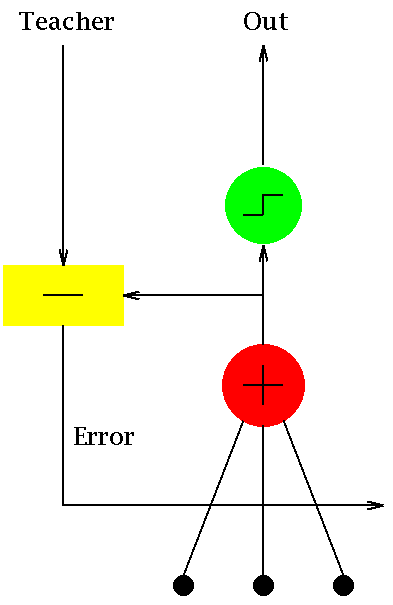
\includegraphics[scale = 0.3]{lectures/4_neural_networks/4_Adaline_flow_chart.png}
        \caption{Learning inside a single layer ADALINE}
        \label{fig:4_Adaline_flow_chart}
    \end{figure}
    
    This net is linear,  LMS direct solution and gradient descent solution. Adeline infact is in also know as Delta rule, Least mean square or Widrow- Hoff.
    \begin{itemize}
        \item Regression tasks: See the LMS algorithm
        \item For classification: See the LTU and LMS algorithm of a previous lectures (on linear model)
        \item An approach that we will generalize to MLP
    \end{itemize}
    \item \textbf{Perceptron}: (Rosenblatt): non-linear (with hard limiter or Threshold activation function)
    \begin{itemize}
        \item Only classification: can rappresent a linear decision boundaries (see LTU) of only  linearly separable problems and is always able to learn it: convergence theorem
    \end{itemize}
\end{itemize}

The difference between Adaline and the standard (McCulloch–Pitts) perceptron is that in the learning phase, the weights are adjusted according to the weighted sum of the inputs (the net). In the standard perceptron, the net is passed to the activation (transfer) function and the function's output is used for adjusting the weights.

\subsubsection{The Perceptron Learning Algorithm}
Although we are interested in learning networks of many interconnected units, let us begin by understanding how to learn the weights for a single perceptron. Here the precise learning problem is to determine a weight vector that causes the perceptron to produce the correct output ($\pm 1$) for each of the given training examples:
\begin{itemize}
    \item find $\bold{w}$ such that $sign(\bold{wx})=d$
    \item On-line algorithm: a step can be made for each input pattern
\end{itemize}

\begin{figure}[H]
    \centering
    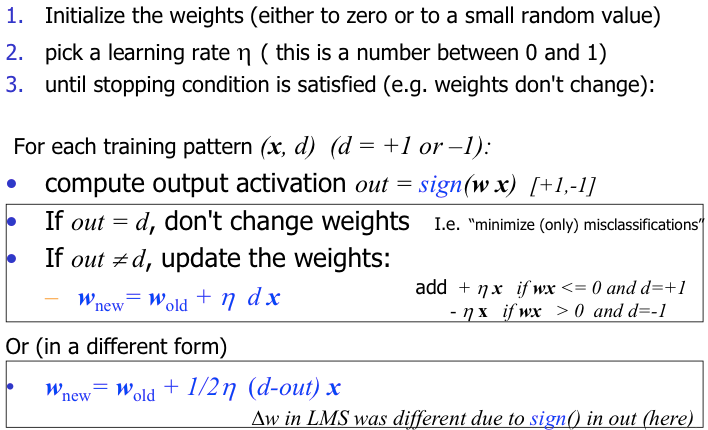
\includegraphics[scale = 0.4]{lectures/4_neural_networks/4_PLA.png}
    \label{fig:pla}
\end{figure}

\noindent$\blacksquare$ \textbf{Geometrical view}\\
An example: Before updating the weight $\mathbf{w}$, we note that both $p1$ and $p2$ are incorrectly classified (red dashed line is decision boundary).
Suppose we choose p1 to update the weights as in picture below.
$p1$ has target value $t = 1$, so that $\mathbf{w}$ is moved a small amount in the direction of $p1$. The new boundary (blue dashed line) is better than before, (and $w_new$ closer to $p1$). Exercise: what happens if the training pattern $p2$ is chosen ? same thing!
\begin{figure}[H]
    \centering
    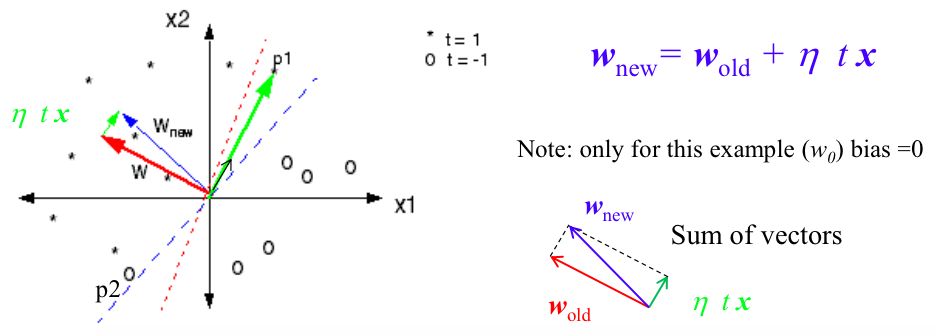
\includegraphics[scale = 0.35]{lectures/4_neural_networks/4_geometrical_view.png}
    \label{fig:geometrical_view}
\end{figure}

\noindent$\blacksquare$ \textbf{Perceptron Learning Algorithm and Delta Rule}\\
\noindent The Perceptron Learning rule can be posed also into delta rule form (using
+1,-1 encoding for the two classes) to show similarity and differences with Delta/ Widrow- Hoff/Adaline/LMS rule.
$$\bold{w}_{new} = \bold{w}_{old} + \eta (d-out)\bold{x}$$
This is an \emph{error-correction} rule (already seen in LMS section) that change the $\bold{w}$ proportionally to the error ($\delta = d-out$).
Weights are modified at each step as happens in \textbf{delta rule}, which revises the weight $w$ associated with input $x$ according to the rule
($\delta = d-out$) where $d$ is the target output for the current training example, $out$ is the output generated by the perceptron and $eta$ is a positive constant called the \emph{learning rate}. The role of the learning rate is to moderate the degree to which weights are changed at each step. It is usually set to some small value (for example 0.1) and is sometimes made to decay as the number of weight-tuning iterations increases.\\

\noindent\textbf{Note}: In terms of “neurons”: the adjustment made to a synaptic weight is proportional to the product of error signal and the input signal that excite the synapse\\


\subsubsection{Perceptron Convergence Theorem}
The Perceptron can represent linear decision boundaries (see LTU) and can solve linearly separable problem.\\
Can it always \emph{learn} the solution?\\
Yes! The Perceptron with the \emph{“Perceptron Learning Algorithm”} is always able to learn what it is able to represent: \emph{Perceptron Convergence Theorem}.\\
\newline
\textbf{Theorem}: \emph{The perceptron is guaranteed to converge (classifying correctly all the input patterns) in a finite number of steps if the problem is linearly separable.}\\

\noindent$\Rightarrow$\textbf{preliminaries}:\\
Let's suppose to have a Training Set: $(\mathbf{x}_i, d_i)$ where $d_i = +1$ or $-1$. Now, we focus only on the \textit{Positive patterns} with $d_i = +1$. If we have two classes that are linearly separable we will have:
$$ \text{Linearly separable }\rightarrow \exists \; \mathbf{w}^* \text{ solution s.t. } d_i(\mathbf{w^*}\mathbf{x}_i) \geq \alpha$$
$$ \alpha = \min_i d_i(\mathbf{w^*}\mathbf{x}_i) > 0$$
Hence, $\mathbf{w^*}(d_i\mathbf{x}_i) \geq \alpha$\\
\noindent Defining $x^{'}_{i} = (d_i\mathbf{x}_i)$, then $\mathbf{w}^*$ is a solution iff $\mathbf{w^*}$ is a solution of $(x^{'}_{i}, +1)$\\

\noindent(if) $\mathbf{w^*}$ solve $\rightarrow d_i(\mathbf{w^*}\mathbf{x}_i) \geq \alpha \rightarrow \mathbf{w^*}(d_i\mathbf{x}_i) \geq \alpha \rightarrow (\mathbf{w^*}\mathbf{x}_i) > \alpha \rightarrow \mathbf{w}^*$ is a solution of $(x^{'}_{i}, +1)$\\
(only if)  $\mathbf{w^*}$ is a solution of $(x^{'}_{i}, +1) \rightarrow (\mathbf{w^*}d_i\mathbf{x}_i) \geq \alpha \rightarrow  d_i(\mathbf{w^*}\mathbf{x}_i) \geq \alpha \rightarrow \mathbf{w^*}$ solve for $\mathbf{x}_i$\\

Now let's assume that at step $0$: $\mathbf{w(0)} = 0$ and $\eta = 1, \beta = \max_i \norm{\mathbf{x}_i}^2$

After q errors (all false negative, the perceptron incorrectly classifies it:
$$\mathbf{w}(q) = \sum_{j=1}^{q} \mathbf{x}_{i_j} \;,\; \text{because } \mathbf{w}(j) = \mathbf{w}(j-1) + \mathbf{x}_{i_j}$$

\textbf{Note:} $\bold{w}_{new} = \bold{w}_{old} + \eta (d)\bold{x}$ but all $d$ are $+1$ here, we are considering only positive patterns.\\

\noindent$\Rightarrow$\textbf{Proof}:\\
we can find lower and upper bound to $\norm{\mathbf{w}}|$ as a function of $q^2$ steps (lower bound) and $q$ steps (upper bound) $\rightarrow$ we can find $q$ s.t. the
algorithm converges.

\begin{itemize}
    \item Lower bound on $\norm{\mathbf{w}(q)}$:
        $$ \mathbf{w^*w}(q) = \mathbf{w^*}\sum_{j = 1}^{q} \mathbf{x}_{i_j} \geq q\alpha \;\;,\;\; \alpha = \min_i (\mathbf{w^*}\mathbf{x}_i)$$
        
        We make use of an inequality known as the Cauchy–Schwarz inequality: 
        $$(\mathbf{wv})^2 \leq \norm{\mathbf{w}^2}\norm{\mathbf{v}^2} \text{  (Cauchy–Schwarz)}$$
        So we can write:
        $$ \norm{\mathbf{w^*}}^2\norm{\mathbf{w}(q)}^2 \geq (\mathbf{w^*w}(q))^2 \geq (q\alpha)^2$$
        the lower bound is:
        $$ \norm{\mathbf{w}(q)}^2 \geq \frac{(q\alpha)^2}{\norm{\mathbf{w^*}}^2}$$
        
    \item Upper Bound on $\norm{\mathbf{w}(q)}$:
    \begin{center}
        we know that $\norm{\mathbf{a}+\mathbf{b}}^2 = \norm{a}^2 +2\mathbf{ab} + \norm{b}^2$, so we can write:
    \end{center}
    $$ \norm{\mathbf{w}(q)}^2 = \norm{\mathbf{w}(q-1)+ \mathbf{x}_{i_q}}^2 = \norm{\mathbf{w}(q-1)}^2  + 2\mathbf{w}(q-1)\mathbf{x}_{i_q} +\norm{\mathbf{x}_{i_q}}^2 $$ 
    
    But for the q-th error, $\mathbf{w}(q-1)\mathbf{x}_{i_q} \leq 0$.  We therefore deduce that:
    $$ \norm{\mathbf{w}(q)}^2 \leq  \norm{\mathbf{w}(q-1)}^2 +\norm{\mathbf{x}_{i_q}}^2$$
    invoking the assumed initial condition $\mathbf{w}(0) = 0$, we get the upper bound:
    $$ \norm{\mathbf{w}(q)}^2 \leq \sum_{j = 1}^{q} \norm{\mathbf{x}_{i_j}}^2 \leq q\beta \; , \; \beta = \max_i \norm{\mathbf{x}_i}^2$$
\end{itemize}
Let's put all together:
$$ q\beta \geq \norm{\mathbf{w}(q)}^2 \geq \frac{(q\alpha)^2}{\norm{\mathbf{w^*}}^2}$$ 
$$ q\beta \geq q^2\alpha^{'}$$
$$ \beta \geq q\alpha^{'}$$
$$ q \leq \frac{\beta}{\alpha^{'}}$$

\begin{figure}[H]
    \centering
    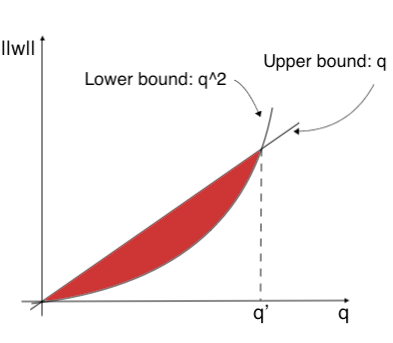
\includegraphics[scale = 0.4]{lectures/4_neural_networks/4_placp.png}
    \caption{Lower and Upper bound}
    \label{fig:4_placp}
\end{figure}

We have thus proved that for $\eta = 1$ and $\mathbf{w}(0) = 0$, and given that a solution vector $\mathbf{w^*}$ exists, the rule for adapting the synaptic weights of the perceptron must terminate after at most $q$ interations. Surprisingly, this statement, proved for positive patterns, also holds for negative patterns.


\subsubsection{Differences between “Perc. Learning Alg.” and LMS Alg.}
$$\bold{w}_{new} = \bold{w}_{old} + \eta (d-out)\bold{x}$$
\begin{itemize}
    \item LMS rule derived without threshold activation functions: minimize the error of the linear unit (using directly $\bold{wx}$)
    \item Hence, for training:
    \begin{center}
        LMS has $\delta=(d-\bold{wx})$ and PLA has $\delta=(d-sign(\bold{wx}))$
    \end{center}
    Of course the model trained with LMS can still be used for classification applying the threshold function $h(x)= sign(\bold{wx})$ (\textbf{LTU})
    
    \item LMS not necessarily minimize the number of TR example misclassified by LTU, see Fig~\ref{fig:misclassify}.
    $$ E(\mathbf{w}) = \sum_{i}^{} (y_i - \mathbf{x}^{T}_{i}\mathbf{w})^2$$
    It changes the weights not only for the misclassified patterns.
    \begin{figure}[h]
        \centering
        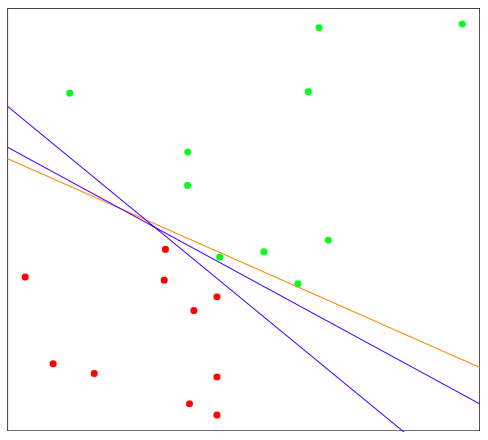
\includegraphics[scale = 0.3]{lectures/4_neural_networks/4_LMS_PLA.png}
        \caption{A toy example with two classes separable by a hyperplane. The orange line is the least squares solution, which misclassifies one of the training points. Also shown are two blue separating hyperplanes found by the perceptron learning algorithm with different random starts.}
        \label{fig:misclassify}
    \end{figure}
    
    \item PLA if training examples are linearly separable, it always converges (after a finite number of iterations) to a perfect classifier, otherwise it not.
    
    \item LMS-(gradient-descent) converges \emph{asymptotically}, regardless of whether the training data are linearly separable (hence even if they are not linearly separable).

\end{itemize}

\textbf{Note}: 
\begin{itemize}
    \item Delta rule for linear unit $\rightarrow$ it minimize the Meand Square (MS) loss.
    \item “Perc. Learning Alg” $\rightarrow$ it has been posed also into delta rule form (using
+1,-1 encoding for the two classes) to show similarity and differences.
\end{itemize}
\newpage

\subsection{Activation functions}
In artificial neural networks, the activation function of a node defines the output of that node given an input or set of inputs. However, only nonlinear activation functions allow such networks to compute nontrivial problems. This function is also called the transfer function.
\subsubsection{Linear function}
    $$ o = net = h(\mathbf{x}) = \sum_{i}^{} w_ix_i$$
    \begin{figure}[H]
        \centering
        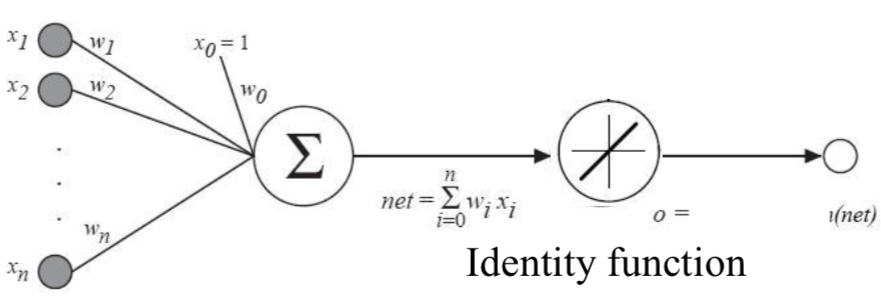
\includegraphics[scale = 0.3]{lectures/4_neural_networks/4_activation_function_linear_act.png}
    \end{figure}
\subsubsection{Threshold (or step) function (Perceptron/LTU)}
    $$ o = \sigma(net) =  sign(net)$$
    \begin{figure}[H]
        \centering
        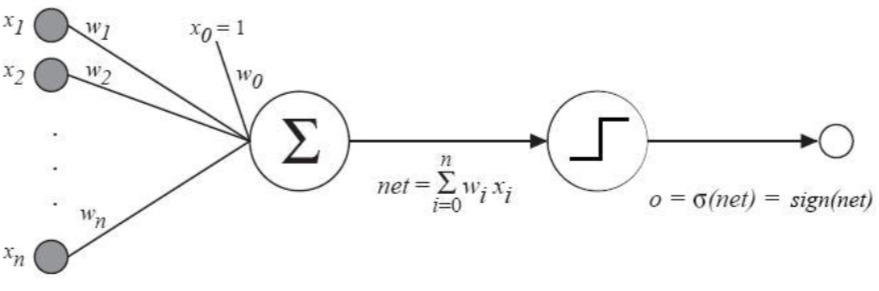
\includegraphics[scale = 0.3]{lectures/4_neural_networks/4_activation_function_ltu.png}
    \end{figure}
\subsubsection{Sigmoidal logistic Function}
A non-linear squashing function like the sigmoidal logistic Function: assumes a continuous range of values in bounded interval [0,1].
    \begin{figure}[H]
        \centering
        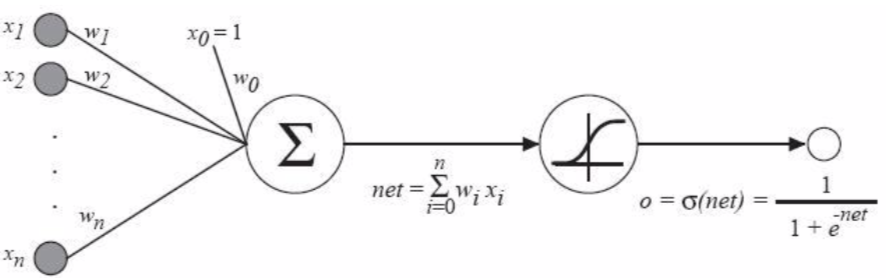
\includegraphics[scale = 0.3]{lectures/4_neural_networks/4_activation_function_sigmoid.png}
    \end{figure}
$$ f_{\sigma}(x) =  \frac{1}{1 - e^{-ax}}$$
The sigmoidal-logistic function has the property to be a smoothed differentiable threshold function. $a$ is the slope parameter of the sigmoid function.
\begin{figure}[H]
    \centering
    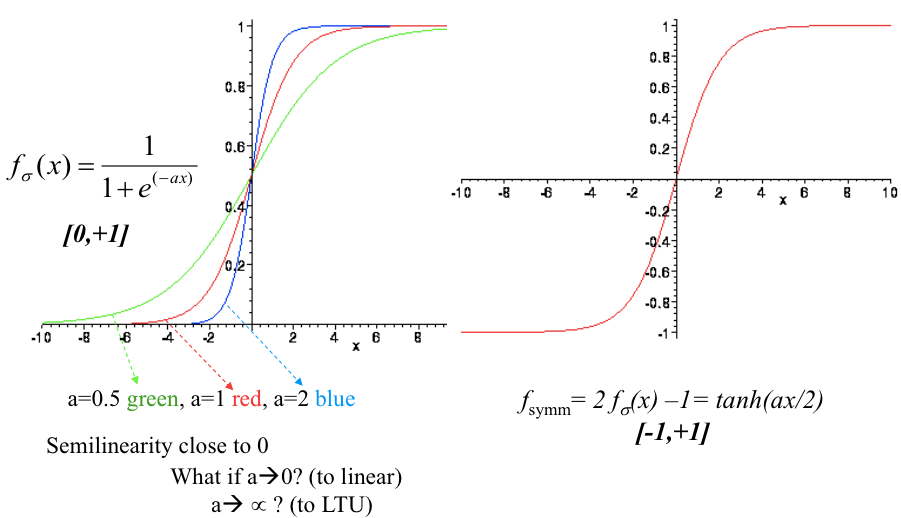
\includegraphics[scale = 0.4]{lectures/4_neural_networks/4_act_func_sig_two.png}
\end{figure}

\subsubsection{Other Activation Functions}
\noindent$\blacksquare$ \textbf{Radial Basis Functions}\\
Radial Basis Functions $\rightarrow$ RBF networks
\begin{figure}[H]
    \centering
    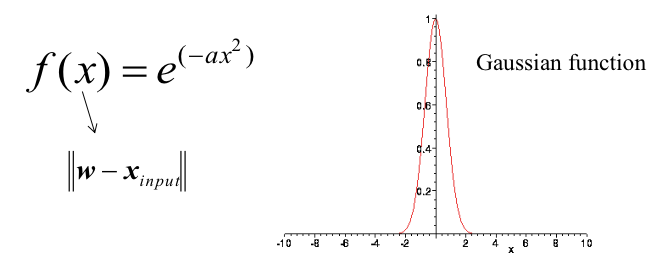
\includegraphics[scale = 0.4]{lectures/4_neural_networks/4_Radial_Basis_Functions.png}
\end{figure}

\noindent$\blacksquare$ \textbf{Softmax}\\
see next lectures (multi-output case)\\

\noindent$\blacksquare$ \textbf{Stochastic neurons}\\
output is $+1$ with probability $P(net)$ or $–1$ with $1-P(net)\rightarrow$ Boltzmann machines and other models rooted in statistical mechanics.\\

\noindent$\blacksquare$ \textbf{Tanh-like}\\
Tanh-like (piecewise linear approximation) for efficient computation. $n$ steepness (slope) of the function Rounding operator (floor)
Shift operation in binary rep.
$$ f(x) = sign(x)\left[ 1 + \frac{1}{2^{\lfloor 2^n \abs{x} \rfloor}} \left( \frac{2^n\abs{x}- \lfloor 2^n \abs{x}\rfloor}{2}-1 \right) \right]$$

\noindent$\blacksquare$ \textbf{ReLU (Rectified Linear Unit)}\\
Rectifier $\rightarrow$ ReLU (Rectified Linear Unit): see Deep Learning section. It became a default choice for Deep models, so it (and its variants) deserves more attention discussing Deep Learning.
\[
    f(x) = \left\{
                \begin{array}{ll}
                  0 \quad for \;\; x<0\\
                  x \quad for \;\; x \geq 0
                \end{array}
              \right.
\]
$$ f(x) = \max(0,x) $$
\begin{figure}[H]
    \centering
    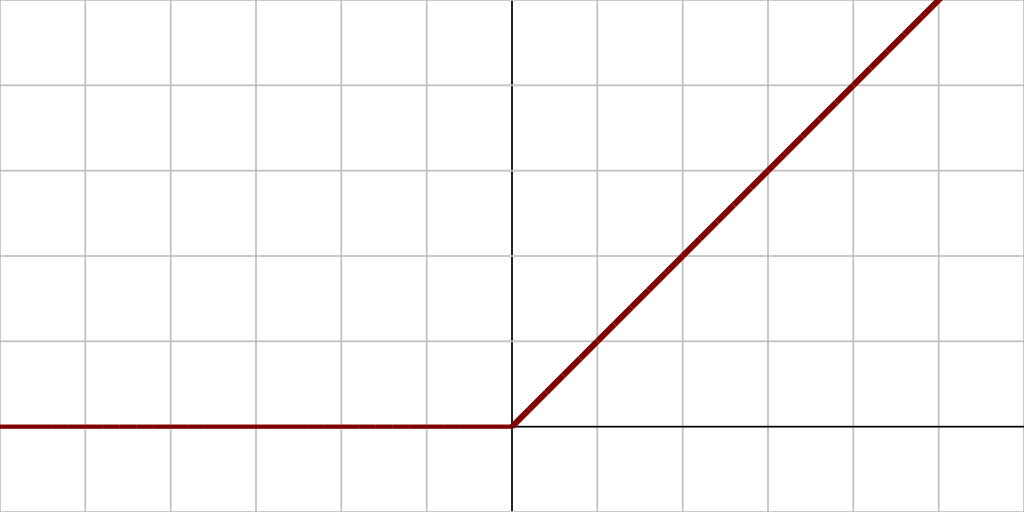
\includegraphics[scale = 0.15]{lectures/4_neural_networks/4_relu.png}
    \caption{Relu activation function}
    \label{fig:4_relu}
\end{figure}
\noindent$\blacksquare$ \textbf{Softplus (smooth approximation)}\\
$$ f(x) = ln(1 + e^x)$$
\begin{figure}[H]
    \centering
    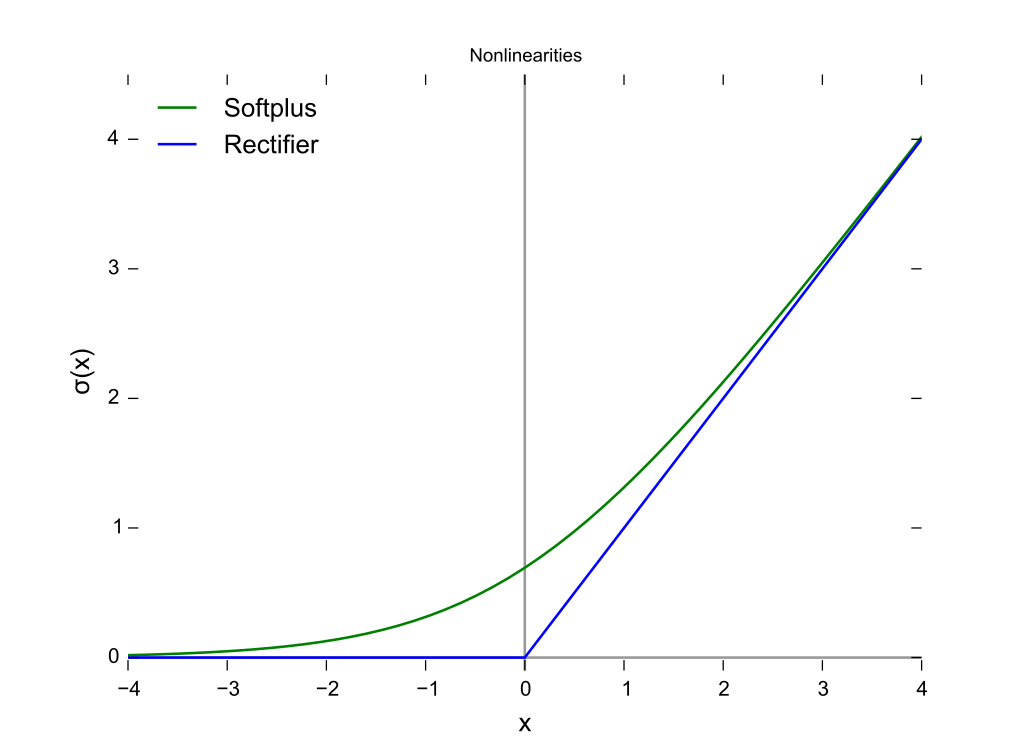
\includegraphics[scale = 0.22]{lectures/4_neural_networks/4_softplus.png}
    \caption{Softplus (smooth approximation)}
    \label{fig:4_softplus}
\end{figure}

\subsubsection{Activation functions: derivatives}
\begin{itemize}
    \item The derivative of the identity function is 1.
    \item The derivative of the step function is not defined which is exactly why it isn't used.
    \item Sigmoids: for asimmetric and simmetric case we have $(a=1)$:
    $$ \frac{d f_\sigma (x)}{dx} = f_\sigma(x)(1 - f_\sigma (x)) \quad\quad\quad \frac{d f_{tanh} (x)}{dx} = 1 - f_{tanh}^2$$
    this is true also with any a.
\end{itemize}

\subsection{Least Mean Square with Sigmoids}
The sigmoidal-logistic function has the property to be a smoothed differentiable threshold function. Hence, we can derive a Least (Mean) Square algorithm by computing the gradient of the loss function as for the linear units (also for a classifier).\\

From $o(\mathbf{x})= \mathbf{xw}$ to $o(\mathbf{x})=f_\sigma(\mathbf{xw})$ where $f_\sigma$ is a logistic function and we want to find $\mathbf{w}$ to minimize the residual sum of squares:
$$ E(\mathbf{w}) = \sum_{p}^{}(d_p - o(\mathbf{x}_p))^2 = \sum_{p}^{} (d_p - f_\sigma(\mathbf{x_p^Tw}))^2$$

\noindent$\blacksquare$  \textbf{LMS with 1 non-linear unit}:\\
The algorithm is always the same, gradient descent algorithm (batch or online), for the Delta rule we have to compute the gradient of the loss.
$$\frac{\partial E_p(\mathbf{w})}{\partial\mathbf{w}_i}\;,\quad \quad \quad o(\mathbf{x}_p) = out(\mathbf{x}_p)  = f_\sigma(\mathbf{xw})$$
Now we want to compute $\frac{\partial E(\mathbf{w})}{\mathbf{w}_j}$:
$$\frac{\partial E(\mathbf{w})}{\partial \mathbf{w}_j} = \frac{ \sum_{p}^{} \partial(d_p - f_\sigma(\mathbf{x}_{p}^{T}\mathbf{w}))^2}{\partial \mathbf{w}_j}\;\;,\;\; net = \mathbf{x}_p^T \mathbf{w}$$
$$ \frac{\partial E(\mathbf{w})}{\partial \mathbf{w}_j} = \frac{\partial E(\mathbf{w})}{\partial net}\frac{\partial net}{\partial \mathbf{w}_j} = \frac{ \sum_{p}^{} \partial(d_p - f_\sigma(net))^2}{\partial \mathbf{w}_j} \frac{\partial net}{\partial \mathbf{w}_j}\;\;,\;\; out = f_\sigma(net) $$

$$  \frac{\partial net}{\partial \mathbf{w}_j} = \frac{\partial \sum_{t = 0}^{n} w_t x_{p,t}}{\partial \mathbf{w}_j}  = (x_p)_j$$
$$  \frac{\partial E(\mathbf{w})}{\partial net} = \frac{\partial E(\mathbf{w})}{\partial out} \frac{\partial out}{\partial net} = \frac{ \sum_{p}^{} \partial(d_p - out)^2}{\partial out} f^{'}_\sigma(net) =$$ 
$$= 2\sum_{p}^{}(d_p - out) \frac{\partial(d_p - out)}{\partial out}  f^{'}_\sigma(net) = -2\sum_{p}^{}(d_p - out)f^{'}_\sigma(net)$$
by put all together we can find:
$$\frac{\partial E_p(\mathbf{w})}{\partial\mathbf{w}_i} = -2\sum_{p}^{}(d_p - f_\sigma(net))f^{'}_\sigma(net)(x_p)_j = -2\sum_{p}^{}(x_p)_j \delta_p$$ 

\noindent$\blacksquare$  \textbf{Gradient descent algorithm}:\\
The same as for linear unit using the new delta rule (batch/on-line):
$$ \mathbf{w}_{new} = \mathbf{w}_{old} + \eta\delta_p \mathbf{x}_p\;\; , \;\; \delta_p = (d_p - f_\sigma(net))f^{'}_\sigma(net) \quad \text{(Pattern p)}$$
The unique Unit has not index here.
\begin{figure}[H]
    \centering
    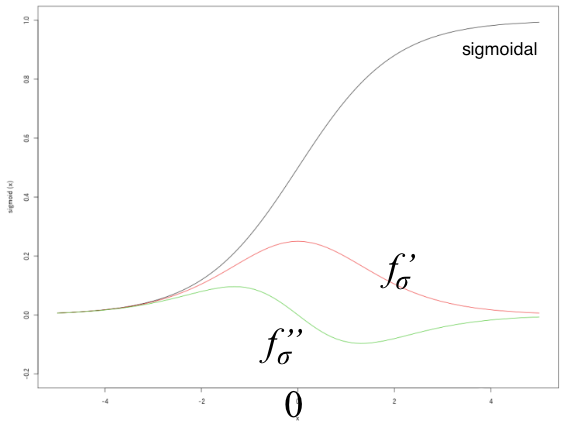
\includegraphics[scale = 0.3]{lectures/4_neural_networks/4_new_delat_rule.png}
    \caption{new delta rule}
    \label{fig:4_new_delat_rule}
\end{figure}
\textbf{Note}:
\begin{itemize}
    \item Again we have an error correction rule, but the new $\delta_p$ it depends on the difference and on the derivative of the sigmoid function.
    
    \item the parameters $a$ of the sigmoid function  can affect the step of gradient descent.
    
    \item Max of $f^{'}$ for input close to $0$ ($\sim$ linear unit).
    
    \item Minimum of  $f^{'}$ is for saturated cases: better start with small weights to avoid saturation, and hence very slow changes of w, at the beginning and use the regularization to lower the weights.
    
    \item Insight: also a bridge between the two algorithm: toward no corrections for correct output also for LMS algorithm.
\end{itemize}

\subsection{Multi-Layer Perceptron (MLP)-NN}
All the ingredients are ready and we can start to talk about Neural Networks. Neural Networks by two views of Multi-Layer Perceptron (MLP)-NN:\\

\noindent E.g. Standard feedforward NN (with one hidden layer):\\

\textbf{1.} A network of interconnected units:\\
 the architectural graph of a multiplayer perceptron with one hidden layers and an output layer. To set the stage for a description of the multilayer percep-tron in its general form, the network shown here is fully connected. This means that a neu-ron in any layer of the network is connected to all the neurons (nodes) in the previous layer (except the input ones). Signal flow through the network progresses in a forward direction, from left to right and on a layer-by-layer basis.
\begin{figure}[H]
    \centering
    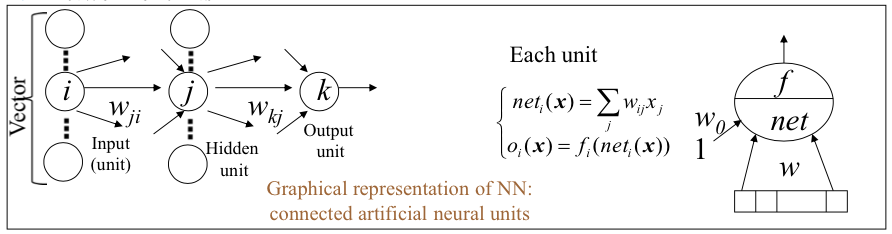
\includegraphics[scale = 0.4]{lectures/4_neural_networks/4_network_of_units.png}
\end{figure}
\textbf{2.} A flexible function $h(x)$ (as nested non-linear functions)
\begin{figure}[H]
    \centering
    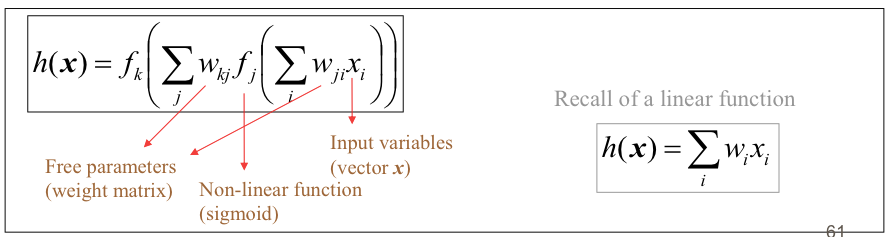
\includegraphics[scale = 0.4]{lectures/4_neural_networks/4_flexible_function.png}
\end{figure}

\noindent$\blacksquare$ \textbf{Neural Networks: components}\\
NN model traditionally presented by the type of:
\begin{itemize}
    \item \textit{UNIT}: net, activation functions
    \item \textit{ARCHITECTURE}: number of units, topology (e.g. also number of layers)
    \item \textit{LEARNING ALGORITHM}
\end{itemize}

The architecture of a NN defines the topology of the connections among the units. E.g \textbf{Feedforward} and \textbf{Recurrent} neural networks.

\subsubsection{MLP Standard feedforward NN}
The two-layer feedforward neural network described in Equation h(x) corresponds to the well-know MLP (Multi Layer Perceptron) architecture:
\begin{center}
    direction: input $\rightarrow$ output
\end{center}

\begin{itemize}
    \item the units are connected by weighted links and they are organized in the form of layers.
    
    \item the input layer is simply the source of the input $\mathbf{x}$ that projects onto the hidden layer of units.

    \item the hidden layer projects onto the output layer (feedforward computation of a two-layer network).
\end{itemize}

\begin{figure}[H]
    \centering
    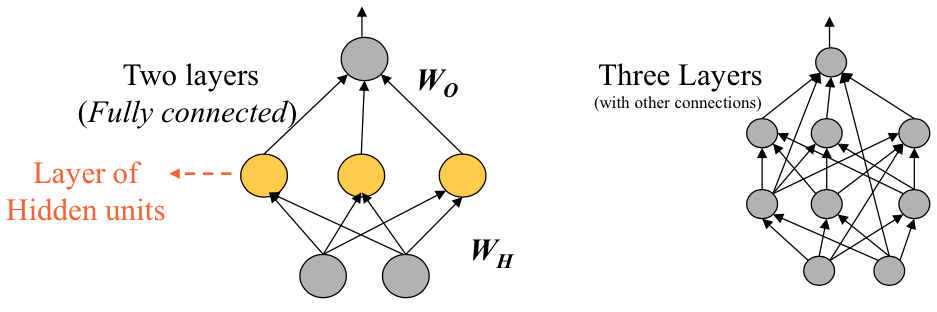
\includegraphics[scale = 0.35]{lectures/4_neural_networks/4_feed_f.png}
    \caption{A feedforward NN on the lef and a Three Layers with other connections NN on the right}
    \label{fig:4_feed_f}
\end{figure}

\subsubsection{Recurrent neural networks}
Recurrent neural networks: A different category of architecture, based
on the addition of feedback loops connections in the network topology:
\begin{itemize}
    \item The presence of self-loop connections provides the network with dynamical properties, letting a memory of the past computations in the model.
    \item This allows us to extend the representation capability of the model to the processing of sequences (and structured data).
\end{itemize}

\begin{figure}[H]
    \centering
    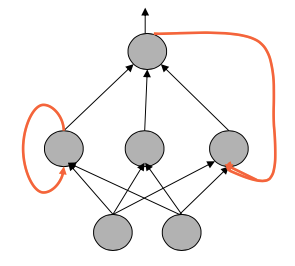
\includegraphics[scale = 0.4]{lectures/4_neural_networks/4_recurrent_nn.png}
    \caption{Recurrent neural networks}
    \label{fig:4_recurrent_nn}
\end{figure}


\subsubsection{Flexibility of Neural Network model}
There are some important questions about neural networks:
\begin{enumerate}
    \item Why NN is a flexible model? why work well? Can be interpreted as linear basis expansion (LBE)?
    \item Is the flexibility theoretically grounded?
\end{enumerate}

\noindent$\blacksquare$ \textbf{Neural Network flexibility}\\
\textbf{Hypothesis space} of a Neural Network: continuous space of all the functions that can be represented by assigning the weight values of the given architecture.

\begin{itemize}
    \item Note that, depending on the class of values produced by the network output units, discrete or continuous, the model can deal, respectively, with classification (sigmoidal output f.) or regression (linear output f.) tasks.
    \begin{figure}[H]
      \centering
      \subfloat[Neural Network]{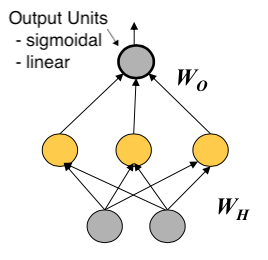
\includegraphics[width=0.40\textwidth, scale = 0.2]{lectures/4_neural_networks/4_nn_flexibility1.png}\label{fig:4_nn_flexibility1}}
      \hfill
      \subfloat[$h(\mathbf{x})$]{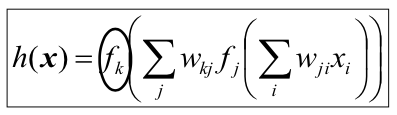
\includegraphics[width=0.45\textwidth]{lectures/4_neural_networks/4_nn_flexibility2.png}\label{fig:4_nn_flexibility2}}
      \caption{A Neural Network can solve regression and classification task.}
    \end{figure}
    \item Also multi-regression or multi-classes classifier can be obtained by using multiple output units
\end{itemize}

\noindent$\blacksquare$ \textbf{Neural Network as a function}\\
\begin{figure}[H]
    \centering
    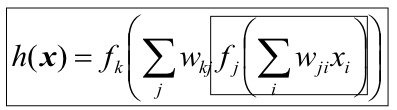
\includegraphics[scale = 0.4]{lectures/4_neural_networks/4_nn_as_function.png}
\end{figure}
\begin{itemize}
    \item This is the function computed by a two-layer feedforward neural network
    \item Units and architecture just a graphical representation (of the data flow process)
    \item each $f_j(\sum_{i}^{}w_{ji}x_i)$, can be seen as computed by an independent processing
element (unit)
\end{itemize}
Indeed, NN is a function non linear in the parameters $w$.\\

\noindent$\blacksquare$ \textbf{Neural Network as a dictionary approach}\\
We have seen in the Least Mean Square the \textbf{linear basis expansion (LBE)}, in that case the phi was preselected and fiexed and does not change with trainig data:
$$ \text{linear with respect to parameters w: } \sum_{j}^{}w_j\phi_j(\mathbf{x})$$
But in NN we have an \textbf{Adaptive(flexible)} basis functions approach, the basis functions themselves are adapted to data (by fitting of w in phi):
$$ h(\mathbf{x}) = f_k\left(\sum_{j}^{}w_{kj}\phi_j(\mathbf{x,w})\right)\;,\;\;\phi_j(\mathbf{x,w}) = f_j\left( \sum_{i}^{}w_{ji}x_i \right)$$
Note that we fix the same type of basis functions for all the terms in the basis expansion (given by the activation function).\\


$h(x)$ as (nonlinear function of weighted) sums of nonlinearly transformed linear models plus the important enhancement of adaptivity\\

\noindent$\blacksquare$ \textbf{Hidden Layer Relevance and Interpretation}\\
Each basis function (\textbf{hidden unit}) compute an a \textbf{new} nonlinear derived features, \textbf{adaptively} by learning, according to the training data. I.e. the parameters of the basis function w are learned from data by learning.
$$\phi_j(\mathbf{x,w}) = f_j\left( \sum_{i}^{}w_{ji}x_i \right)$$
In other words:
\begin{itemize}
    \item The representational capacity of the model is related to the presence of a hidden layer of units, with the use of non-linear activation function, that transforms the input pattern into the \textbf{internal representation} of the network.
    
    \item The learning process can define a \textbf{suitable internal representation}, also visible as new hidden features of data, allowing the model to \textbf{extract from data} the higher-order statistic that are relevant to approximate the target function.
\end{itemize}
$$ h(\mathbf{x}) = f_k\left(\sum_{j}^{}w_{kj} f_j\left( \sum_{i}^{}w_{ji}x_i\right)\right)$$
Non-linear units are essential, MLP with linear units = 1 layer NN!\\

Anyway for the learning algorithm this introduce an issue:
\begin{center}
Non-linear w.r.t. to $w$ $\rightarrow$ non linear optimization problem.
\end{center}

The hidden neurons act as feature detectors; as such, they play a critical role in the operation of a multilayer perceptron. As the learning process progresses across the multilayer perceptron, the hidden neurons begin to gradually “discover” the salient features that characterize the training data. They do so by performing a nonlinear transformation on the input data into a new space called the feature space. In this new space, the classes of interest in a pattern-classification task, for example, may be more easily separated from each other than could be the case in the original input data space. Indeed, it is the formation of this feature space through supervised learning that distinguishes the multilayer perceptron from Rosenblatt’s perceptron.\\

\noindent$\blacksquare$ \textbf{Universal approximation}\\
Many early results (Cybenko 1989, Hornik et al. 1993, etc...)
\begin{itemize}
    \item A single hidden-layer network (with logistic activation functions) can approximate (arbitrarily well) every continuous (on hyper cubes) function (provided enough units in the hidden layer) [e.g. image it generalizes approximation by finite Fourier series]
    
    \item A MLP network can approximate (arbitrarily well) every input- output mapping (provided enough units in the hidden layers)
\end{itemize}
\begin{figure}[H]
    \centering
    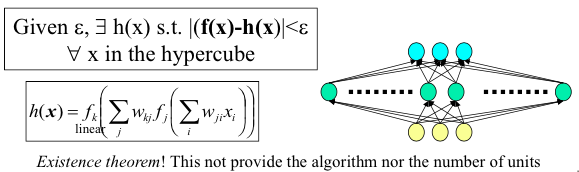
\includegraphics[scale = 0.5]{lectures/4_neural_networks/4_universal_approximation.png}
\end{figure}
After this fundamental result (MLP is able to represent any function), two issues will deserve our attention:
\begin{itemize}
    \item How to learn by NN
    \item How to decide a NN architecture
\end{itemize}

\subsubsection{NN Expressive power}
The \textbf{expressive power} of NN is strongly influenced by two aspects: the number of units and their configuration (architecture).\\

The number of units can be related to the discussion of the VC-dimension of the model.
Specifically, the network capabilities are influenced by the number of parameters, that is proportional to the number of units,
and further studies report also the dependencies on their value sizes, E.g.\\

\noindent Weights = 0 $\rightarrow$ minimal Vc-dim\\
Small weights$\rightarrow$linear part of the activation function\\
Higher weights values$\rightarrow$more complex model\\

\noindent Number of parameters (fully-connected neural network MLP):\\
 \#input-unit * \#hidden-unit * \#output-unit\\

\noindent$\blacksquare$ \textbf{How many layers?}\\
A look ahead (toward \textbf{deep learning}):
\begin{itemize}
    \item The Universal Approximation theorem is a fundamental contribution
    \item It show that 1 hidden layer is sufficient in general, but it does not assure that a “small number” of units could be sufficient (it does not provide a limit on such number)
    \item It is possible to find boundaries on such number (for many f. families)
    \item But also to find “no flattening” results (on efficiency, not expressivity):
    cases for which the implementation by a single hidden layer would require an exponential number of units (w.r.t n input dim.), or non-zero weights, while more layers can help (it can help for the number of units/weights and/or for learning such approximation).\\
    But is it easy to optimize (training) a MLP with many layers? we will see later in deep learning.
\end{itemize}
\newpage
\subsubsection{The Backpropagation Algorithm}
\textbf{How to learn the weights of a NN?}\\
We want a \emph{learning algorithm} that allows adapting the free-parameters of the model in order to obtain the best approximation of the target function.\\
As we saw, in the ML framework this is often realized in terms of minimization of an error (or loss) function on the training data set.\\

\noindent The problem is the same we have seen for the other models (repetita):
\begin{itemize}
    \item \textbf{Given} a set of $l$ training examples $(\bold{x}_p,d_p)$ and a loss function (measure) $L$
    \item \textbf{Find} the weight vector $\bold{w}$ that minimizes  the expected loss on the training data:
    $$E(\bold{w}) = R_{emp} = \frac{1}{l}\sum_{p=1}^{l}L(h(\bold{x}_p),d_p)$$
\end{itemize}
For the \emph{perceptron} we have the \emph{Perceptron learning algorithm (delta rule)}, now we have to define a \textbf{Learning Algorithm for the network (MLP)}.
\begin{figure}[H]
    \centering
    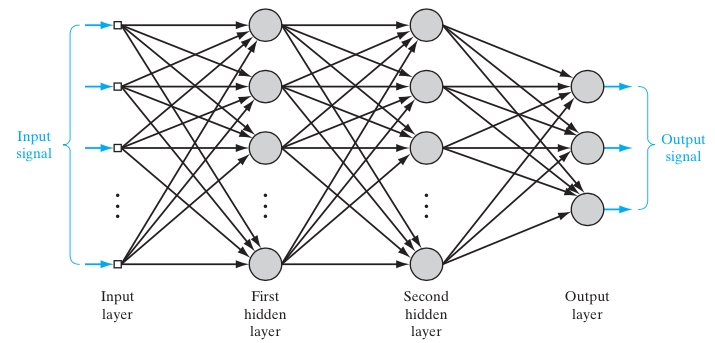
\includegraphics[scale = 0.45]{lectures/4_neural_networks/4_mlp.png}
    \caption{Architectural graph of a multilayer perceptron with two hidden layers.}
    \label{fig:4_mlp}
\end{figure}

\noindent$\blacksquare$ \textbf{Credit assignment problem:}\\
When studying learning algorithms for distributed systems, exemplified by the multilayer perceptron of Figure~\ref{fig:4_mlp}, it is instructive to pay attention to the notion of credit assignment. Basically, the credit-assignment problem is the problem of assigning credit or blame for overall outcomes to each of the internal decisions made by the hidden computational units of the distributed learning system, recognizing that those decisions are responsible for the overall outcomes in the first place.
In a multilayer perceptron using error-correlation learning, the credit-assignment problem arises because the operation of each hidden neuron and of each output neuron in the network is important to the network’s correct overall action on a learning task of interest. That is, in order to solve the prescribed task, the network must assign certain forms of behavior to all of its neurons through a specification of the error-correction learning algorithm. With this background, consider the multilayer perceptron depicted in Fig.~\ref{fig:4_mlp}. Since each output neuron is visible to the outside world, it is possible to supply a desired response to guide the behavior of such a neuron. Thus, as far as output neurons are concerned, it is a straightforward matter to adjust the synaptic weights of each output neuron in accordance with the error-correction algorithm. But how do we assign credit or blame for the action of the hidden neurons when the error-correction learning algorithm is used to adjust the respective synaptic weights of these neurons? The answer to this fundamental question requires more detailed attention than in the case of output neurons.
In what follows in this chapter, we show that the back-propagation algorithm, basic to the training of a multilayer perceptron, solves the credit-assignment problem in an elegant manner.\\
Supposed too difficult by Minsky-Papert (1969), while faced by many researchers (see historical notes) with the back-propagation algorithm popularized by Rumelhart, Hinton, Williams in the PDP book (1986)\\


So, the main problem is the Credit assignment problem, we can use a Gradient descend approach which minimizes a loss function, it can be extended to MLP with the back-propagation algorithm that will be able to change \textbf{the hidden layer weights}.\\

\textbf{(Repetita)} Non-linear with respect to $w \rightarrow$ non linear optimization problem\\

\noindent$\blacksquare$ \textbf{The loading problem}\\
\textbf{Loading problem}: “loading” a given set of tr data into the free parameters of the Neural Networks
\begin{itemize}
    \item given a network and a set of examples
    \item answer yes/no: is there a set of weights so that the network will be consistent with the examples?
\end{itemize}
The loading problem is NP-complete (Judd, 1990), this implies that hard problems cannot be “solved”.\\

In practice networks can be trained in a reasonable amount of time (for example with the use of the back-propagation algorithm) although optimal solution is not guaranteed.\\

\newpage
\noindent$\blacksquare$ \textbf{Intro to Backpropgation}\\
\emph{Gradient descend approach}, minimizing a loss function, can be extended to MLP. We need a differentiable loss function, differentiable activation functions and a network to follow the information flow.\\

\noindent So we want to \textbf{find $\bold{w}$ by computing the gradient of the loss function}
$$E(\bold{w})=\sum_{p}(d_p-h(\bold{x}_p))^2$$
Here some useful definitions for backpropagation and future topics:
\begin{itemize}
    \item \textbf{Batch}: you divide the dataset into a number of \emph{batches}
    \item \textbf{Batch size}: total number of training examples present in a single batch
    \item \textbf{Epoch}: one epoch is when an entire dataset is passed forward and backward through the neural network only once (an entire cycle of training pattern presentation)
    \item \textbf{Iterations}: Is the number of batches needed to complete one epoch
\end{itemize}
Some nice properties (also for programming):
\begin{itemize}
    \item easy because of the compositional form of the model
    \item keep track only of quantities local to each unit (by local variables) $\rightarrow$ modularity of the units is preserved
\end{itemize}

\noindent$\blacksquare$ \textbf{The Back-propagation based learning algorithm}
\begin{figure}[H]
    \centering
    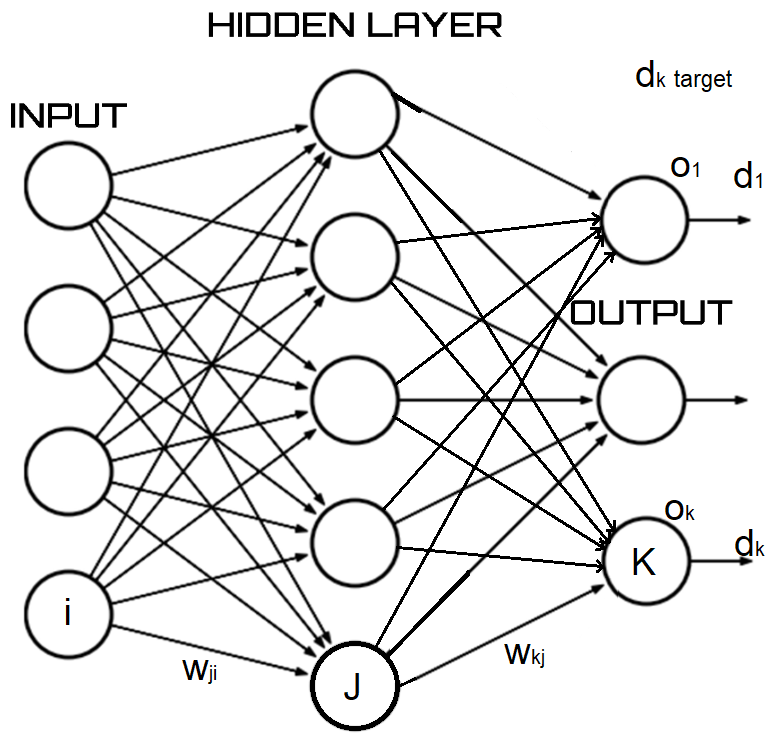
\includegraphics[scale = 0.3]{lectures/4_neural_networks/4_bpa.png}
    \caption{Feed forward fully connected neural network (MLP)}
    \label{fig:4_bpa}
\end{figure}
\begin{itemize}
    \item Training Set = $\{(x^1,d^1),...,(x^i,d^i) \}$
    \item $E_{tot} =\sum_{p}E_p$ where $E_p = \frac{1}{2}\sum_{k} (d_k-o_k)^2$ (for pattern $p$)
    \item Find the $\bold{w}$ parameters such that $min \, E_{tot}$
    \item by Least Mean Square
    \item Descent on the surface E on the basis of the gradient
    \begin{figure}[H]
        \centering
        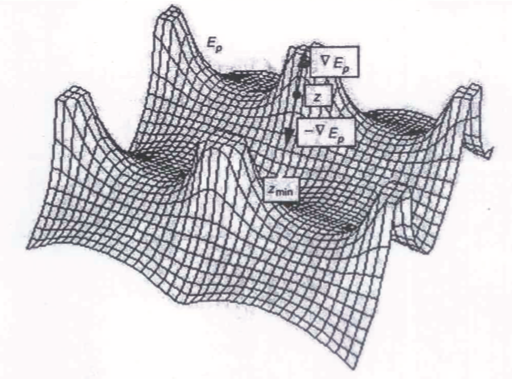
\includegraphics[scale = 0.4]{lectures/4_neural_networks/4_bpalgo_gradient.png}
        \caption{ Example of $E$ in the space of two weights ($w_1$ and $w_2$); the local gradient is shown in the point $Z$. Along the direction of (-gradient) we can reach the $Z_{min}$ point.}
        \label{fig:4_bpalgo_gradient}
    \end{figure}
\end{itemize}
\textbf{Back-propagation}
As mentioned, this backpropagation is based on the \emph{iterative gradient descent algorithm}:\\
Loss function (Error E) $\rightarrow$ gradient computation $\rightarrow$ update the weights $W$
\begin{figure}[H]
    \centering
    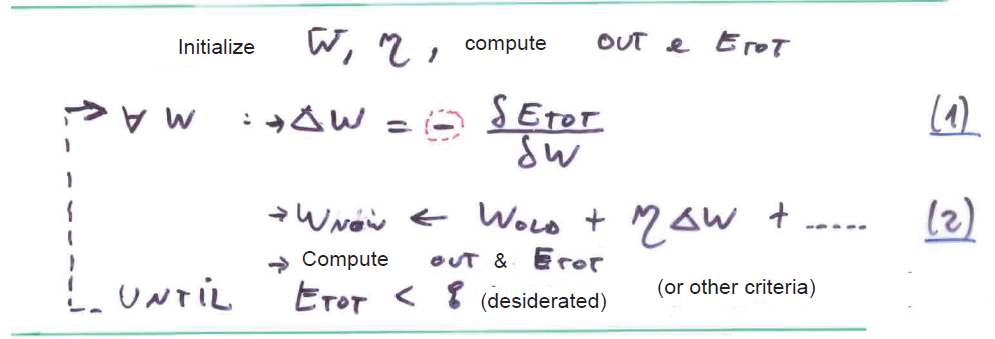
\includegraphics[scale = 0.5]{lectures/4_neural_networks/4_gradient_alg.png}
    \label{fig:4_gradient_alg_backpro}
\end{figure}
\begin{enumerate}
    \item Gradient computation: $\frac{\partial E}{\partial w}$
    \item Upgrade rule for $w$, there many: Standard back-propagation, quick-prop, R-prop, $\dots$
\end{enumerate}
\noindent \textbf{We focus on step (1) - Gradient computation}\\
$$\Delta w = - \frac{\partial E_{tot}}{\partial w} = - \sum_{p} \frac{\partial E_p}{\partial w} = \sum_{p} \Delta_{p}w$$
Where $p$ refers to the p-th pattern feeding in input the neural network.\\

\noindent For the generic unit $t$:
$$\Delta_{p} w_{ti} = - \frac{\partial E_{p}}{\partial w_{ti}} = - \frac{\partial E_{p}}{\partial net_t} \cdot \frac{\partial net_t}{\partial w_{ti}} = \delta_{t} \cdot o_i$$
Where, assuming for pattern $p$, $\delta_t$ is the delta of unit $t$ and $o_i$ is the  input $i$ from a generic unit ($o_i$) to the unit $t$, since
\[
    \left\{
        \begin{array}{ll}
            net_t = \sum_{j} w_{tj}o_j\\
            o_t = f_t(net_t)
        \end{array}
    \right.
    \Rightarrow
    \frac{\partial \sum_{j} w_{tj}o_j}{\partial w_{ti}} = o_i
\]
$o_j\rightarrow$ input $j$ from a generic unit ($o_j$) to the unit t\\
$o_i\rightarrow$ all $0$ except for $j=i$\\

\noindent Now we see the development of $\delta_t$, the error term associated with unit $t$:

$$\delta_t = - \frac{\partial E_p}{\partial net_t} = - \frac{\partial E_p}{\partial o_t} \cdot \frac{\partial o_t}{\partial net_t} = - \frac{\partial E_p}{\partial o_t} \cdot f'_t(net_t)$$
Where $- \frac{\partial E_p}{\partial o_t}$ changes according to the type of unit:

\begin{figure}[H]
    \centering
    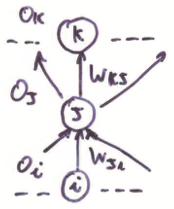
\includegraphics[scale = 0.4]{lectures/4_neural_networks/4_computation_graph_backProp.png}
    \caption{Use the network graph to localize the computation (here by indices)}
    \label{fig:4_computation_graph_backProp}
\end{figure}

\begin{itemize}
    \item \textbf{Out unit K}
    $$- \frac{\partial E_p}{\partial o_k} = - \frac{\partial \frac{1}{2} \sum_{R}(d_R-o_R)^2}{\partial o_k} = (d_k-o_k) \qquad (internal\,\, index\,\, R)$$ $$\Rightarrow \delta_k = (d_k-o_k) \cdot f'_k(net_k)$$
    \item \textbf{Hidden unit J}
    $$- \frac{\partial E_p}{\partial o_j} = \sum_{k} - \frac{\partial E_p}{\partial net_k}\cdot \frac{\partial net_k}{\partial o_j} = \sum_{k} \delta_k \cdot w_{kj}$$ 
    \[
    \text{Since}\left\{
        \begin{array}{ll}
            - \frac{\partial E_p}{\partial net_k} = \delta_k \quad \text{(already computed)}\\
            \frac{\partial net_k}{\partial o_j} = \frac{\partial \sum_{R}^{}w_{kR}o_R}{\partial o_j} = w_{kj}
        \end{array}
    \right.
\]
    
    $$\Rightarrow \delta_j = (\sum_{k}\delta_k w_{kj}) \cdot f'_j(net_j)$$
    It expresses the variation of $E$ with respect to all the output unit $o_k$.\\
    Each $o_k$ (and $net_k$) depends on $o_j$, hence we introduce a sum over $k$.\\
\end{itemize}

\noindent \textbf{Summary}
We derived, for a for a generic unit $t$, with input from $o_i$
$$ \Delta_p w_{ti} = \delta_t o_i$$
\begin{itemize}
    \item IF $t = k$ (output unit)\\
        $$\delta_k = (d_k - o_k)f_k^{'}(net_k)$$
    \item IF $t = j$ (hidden unit)\
        $$\delta_j = \left( \sum_{k}^{}\delta_k w_{kj} \right) f_j^{'}(net_j)$$
\end{itemize}
\begin{figure}[H]
    \centering
    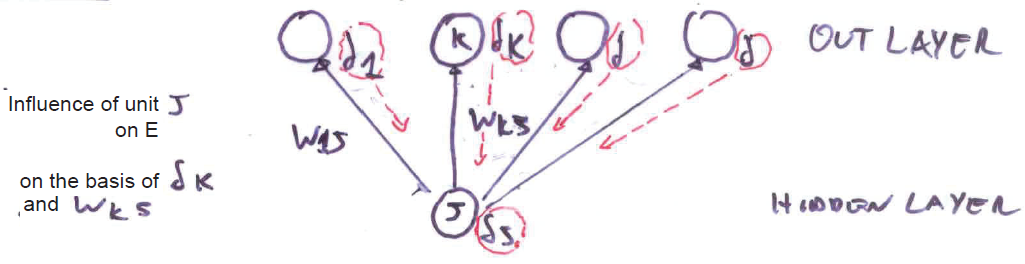
\includegraphics[scale = 0.5]{lectures/4_neural_networks/4_retrop.png}
    \label{fig:4_retrop}
\end{figure}
\noindent\textbf{Retropropagation} of delta ($\delta$) values from the output layer to obtain the error signal for the hidden layers.\\
It can be applied (generalized) to $m$ hidden layers, in other words, deltas come not only from the output layer but also from any generic layer above the current one (a generic upper layer $k$). More in general the deltas come from any units to which this unit is connected to.\\
This will be foundamental for recurrent NN training, for deep learning, etc.
\noindent Hence, for each pattern $p$:
$$w_{ti_{new}} = w_{ti_{old}} + \delta_t o_i$$
Where
\begin{itemize}
    \item $\delta_t$: delta a that level for $t$
    \item $o_i$: input to the unit $t$ from $i$ through the connections $w_{ti}$
\end{itemize}

\textbf{Reference}: Parallel Distributed Processing, Vol.1, by D. E. Rumelhart, J. L. McClelland, MIT Press : Chapter 8 by Rumelhart, Hinton, Williams (1986): \textit{“Learning internal representations by error propagation”}, pages: 322-328.
\subsubsection{Inductive Bias}
What is the inductive bias by which Backpropagation generalizer beyond the observed data? It is difficult to characterize precisely the inductive bias of Backpropagation learning, because it depends on the interplay between the gradient descent search and the way in which the weight space spans the space of representable functions. However, one can roughly characterize it as smooth interpolation between data points.\\

So, Neural Network with backprogation learning algorithm:
\begin{itemize}
    \item Generally related to the \textbf{smoothness} properties of functions we're going to search in the hypothesis space (A very common assumption in ML). E.g a locally limited value of the first derivative.
\end{itemize}
\textbf{Non-smooth} function is generally relative to a random number generator and generalization cannot be achieved.

\newpage
\subsection{Heuristic for the Backpropagation Algorithm}
General problems:
\begin{itemize}
    \item The model is often over-parametrized
    \item Optimization problem is not convex and potentially unstable
\end{itemize}
It is often said that the design of a neural network using the back-propagation algorithm is more of an art than a science, in the sense that many of the factors involved in the design are the results of one’s own personal experience. There is some truth in this statement. Nevertheless, there are methods that will significantly improve the back- propagation algorithm’s performance, as described here. Some of the factors are:
\begin{itemize}
    \item \textbf{Hyperparameters}: Starting values, on-line/batch, learning rate
    \item Multiple Minima
    \item Stopping criteria
    \item Overfitting and regularization
    \item \textbf{Hyperparameters}: Number of hidden units
    \item Input scaling/ Output representation
    \item ...
\end{itemize}

In the previous section we saw that the back-propagation algorithm is essentially the gradient descent algorithm applied to neural networks. The back-propagation is used as a path through the weight space, the path depends on: the data (assumed already given), the neural network model, the starting point (initial weight values) and the final point (stopping rule). This allow to define a control for the search over the Hypothesis space.

\begin{figure}[H]
    \centering
    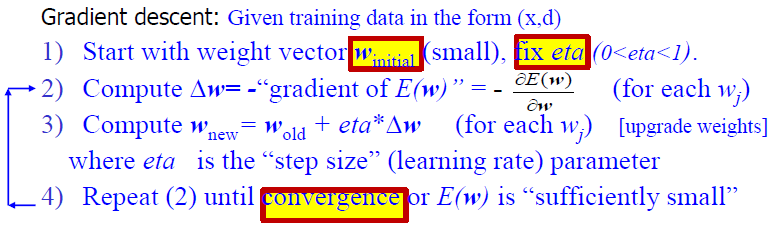
\includegraphics[scale = 0.6]{lectures/4_neural_networks/4_heu.png}
    \label{fig:4_heu}
\end{figure}
But now $\Delta w = -\frac{\partial E(\mathbf{w})}{\partial \mathbf{w}}$ were obtained through back-propagation derivation/algorithm for any weights in the network. At step 2 to compute the Error we first apply inputs to the network computing a forward phase up to the output computation
– then we start the backward phase to retro-propagate the deltas for the gradient.\\

\noindent In this section we discuss few hyperparameters (values that you have to set-up to run the training) of the algorithm, like those highlighted above.\\

\subsubsection{Starting values ($w_{initial}$)}
$\bigstar$ Initialize weights by random values near zero.
Avoid all zero, high values or all equals: these can hamper the training. (for example in \textit{range} [-0.7,+0.7] for standardized data)\\

Other ways:
\begin{itemize}
    \item Considering the Fan-in (the number of inputs to a (hidden) unit), for example $range * 2/fan-in$:
    \begin{itemize}
        \item Not if fan-in is too large
        \item Not for output units (else delta start close to zero!)
    \end{itemize}
    \item Other heuristics... (orthogonal matrix, ...)
    \item Very popular among practitioners: Glorot, Bengio AISTATS 2010:
    0 for biases and $w$ random from Uniform distribution in $[-1/a, +1/a]$ with $a=sqrt(fan-in)$ or (later results) $a$ depending also on fan-out ...
\end{itemize}
\textbf{Note} (practical for the first part of the project): a very small NN (very few units) can have a stronger dependencies w.r.t. initialization.

\subsubsection{Multiple Minima}
The loss function is not \emph{convex}, so we have many \emph{local minima}.

\noindent \underline{But is global minima needed?}\\
\begin{itemize}
    \item Indeed in ML we don’t need neither local or global minima on $R_{emp}$ as we are searching the min of $R$ (that we cannot compute).
    \begin{itemize}
        \item Often we stop in a point that has not null gradient and hence also neither a local or global minima for the empirical (training) error.
    \end{itemize}
    \item The NN build a variable size hp space $\rightarrow$ it increases VC-dim during training $\rightarrow$ the training error decreases toward zero not because we reach a global minimum but because the NN becomes too complex (high VC-dim).\\
    Where \textbf{VC-dim} measures the complexity of the hp space (= flexibility to fit data).
    \item Stopping before this condition of \emph{overtraining} (and hence overfitting) is needed (independently from the issue on local/global minima).
\end{itemize}

\noindent \underline{Multiple Minima are not a big issue}:\\

Multiple Minima are not a big issue because a "good" local minima is often sufficient, you can always see the final training error and check what is happening.\\

The result depends on starting weight values. so the starting weights values help us to find a \emph{good} local minima.\\

\noindent $\bigstar$ Try a number of random starting configurations (for example 10 or more training runs or trials).
\begin{itemize}
    \item Take the \textbf{mean results} (mean of errors) and look to variance to \emph{evaluate} your model and then, if you like to have only 1 response :
    \begin{itemize}
        \item you can choose the solution giving lowest (penalized) error (or the median)
        \item You can take advantage of different end point by an average (committee) response: mean of the outputs/voting
    \end{itemize}
\end{itemize}

\subsubsection{On-line/Batch}
Two versions of \emph{Gradient descent algorithm}.\\
Steps 2 and 3 change to express an inner or external cycle on the patterns:
\begin{figure}[H]
    \centering
    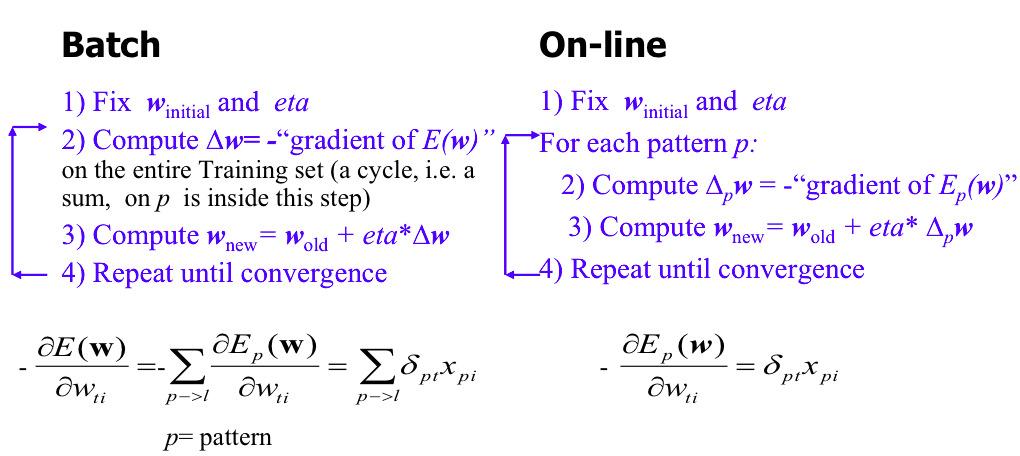
\includegraphics[scale = 0.35]{lectures/4_neural_networks/4_batch_online.png}
    \label{fig:4_batch_online}
\end{figure}
\begin{itemize}
    \item For \textbf{Batch} version: sum up all the gradients of each pattern over an epoch and then update the weights ($\Delta w$ after each “epoch” of $l$ patterns).
    \item \textbf{Stochastic/on-line} version: upgrade $\bold{w}$ for each pattern $p$ (by $\Delta_p w$ ) without wait the total sum over $l$:
    \begin{itemize}
        \item can be faster, but need smaller $\eta$ (\emph{learning rate}): make progress with each examples it looks at.
        \item since the gradient for a single data point can be considered a noisy approximation to the overall gradient, this is also called \textbf{stochastic} (noisy) gradient descent. \emph{Zig-zag (stochastic) descent}.
    \end{itemize}
    \item Another variation exists: \textbf{Stochastic Gradient Descent (SGD)} that use \emph{minibatch} (few training examples) for each step of gradient descent.
\end{itemize}
\begin{figure}[H]
    \centering
    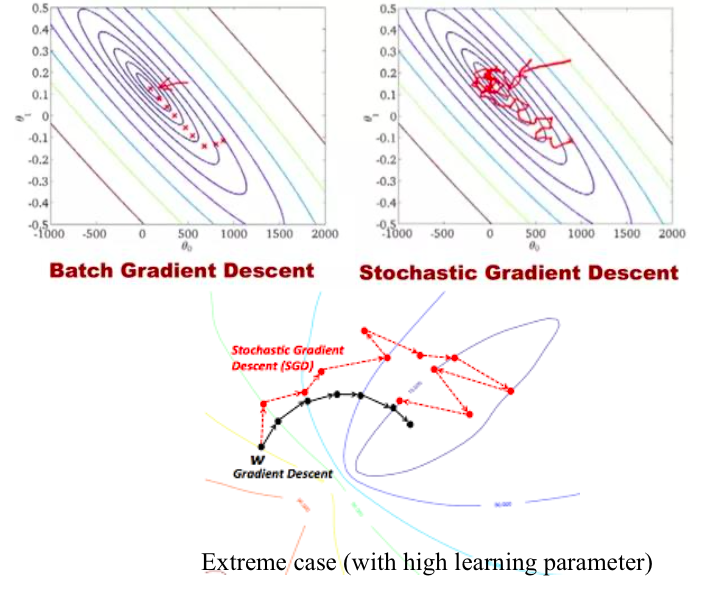
\includegraphics[scale = 0.4]{lectures/4_neural_networks/4_plots_batch_sto.png}
    \caption{Plots stochastics vs batch (with high learning parameter))}
    \label{fig:4_plots_batch_sto}
\end{figure}
Look to the Learning Curve\\
\begin{figure}[H]
    \centering
    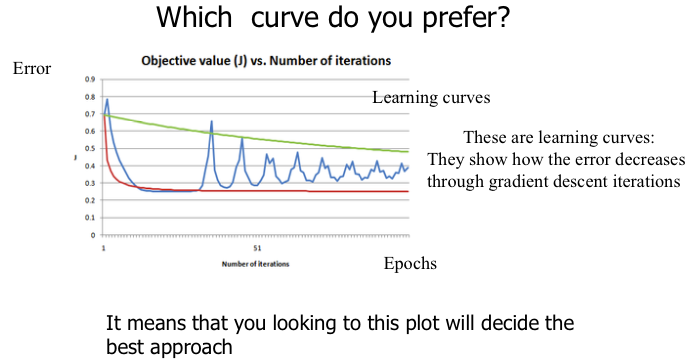
\includegraphics[scale = 0.5]{lectures/4_neural_networks/4_plots_learning_curve.png}
\end{figure}

\subsubsection{Mini-batch SGD}
Mini-batch, with $mb$ examples, to estimate the gradient ($mb$ is the \emph{batch size}).
$$1 < mb < l$$
\begin{itemize}
    \item $mb = 1 \rightarrow$ \emph{Stochastic/on-line}
    \begin{itemize}
        \item cannot exploit parallel processing of examples
        \item may be unstable
        \item can have a regularization effect (adding noise to the learning process), this could be a good side effect.
    \end{itemize}
    \item $mb = l \rightarrow$ \emph{Batch (full training set)}
    \begin{itemize}
        \item more accurate gradient estimation
        \item but slower! (wait all the data)
    \end{itemize}
\end{itemize}
Minibatch stochastic method (SGD):
\begin{itemize}
    \item Use random sampling to implement the minibatch (unbiased estimation). By \emph{shuffling} (at the beginning for all the TR data or for each mini batch)
    
    \item With very large TR set or online streaming $\rightarrow$ even no epochs!
    
    
    \item Along with the advantage of gradient descent (linear cost wrt examples) SGD with $mb$ is a key factor in extending learning to very large data sets (over millions of examples) because $mb$ (and hence the cost of each SGD update) does not depend on $l$ : typically just mini-batch and (again) no epochs repetition
\end{itemize}

\newpage
\subsubsection{Learning rate ($\eta$)}
PREMISE:
\begin{figure}[H]
    \centering
    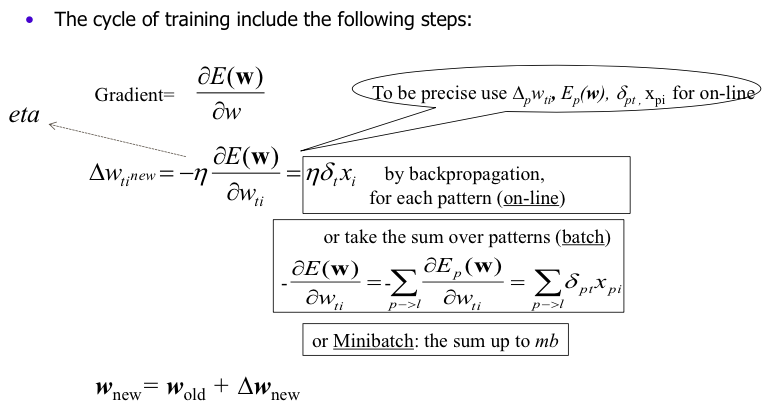
\includegraphics[scale = 0.45]{lectures/4_neural_networks/4_learning_rate_premise.png}
\end{figure}

\noindent Learning rate ($\eta$):
\begin{center}
High versus low eta values: fast versus stable
\end{center}
\begin{itemize}
    \item \textbf{Batch}: more accurate estimation of gradient $\rightarrow$ \textbf{higher $\eta$} (fast).
    \item \textbf{On-line}: use \textbf{smaller value of $\eta$} (stable). This approach can make the training faster and can help avoiding local minima:
    \begin{itemize}
        \item Different order of pattern in different epochs should be used
        \item $\bigstar$ Usually random order (shuffling as already discussed)
    \end{itemize}
\end{itemize}

Some better approaches:
\begin{enumerate}
    \item $\bigstar$ Momentum
    \item Variable learning rate (initially high then decrease)
    \item It can be varied depending on the layer (higher for deep layers) or fan-in (higher for few input connections)
    \item Adaptive learning rates (change during training and for each w) $\rightarrow$ more in Deep Learning.
\end{enumerate}
some possible values fore $\eta = [0.01,\, 0.5]$ in Least Mean Square.\\

\textbf{Practical hints on $\eta$ values}
\begin{itemize}

    \item Too large eta $\rightarrow$ instability, SGD can even increase errors
    
    \item Too small eta $\rightarrow$ not only slow, can even become permanently stuck 
    with high training (TR) error
    
    \item \textbf{Learning curves}, plotting errors during training, allow you to check the behavior in the early phases of the model design for your task at hand (preliminary trials).\\
    $\bigstar$ Please check the Learning Curve training a NN!
    \begin{figure}[H]
        \centering
        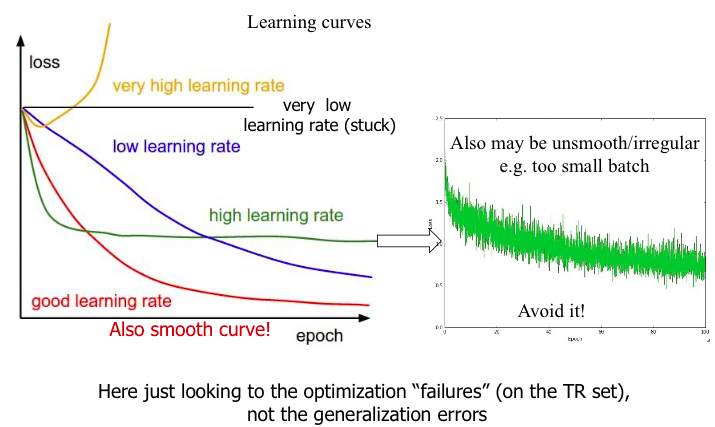
\includegraphics[scale = 0.44]{lectures/4_neural_networks/4_learning_curves.png}
    \end{figure}
    
    \item Of course the absolute value for training error depend also on the model capacity (see later for the number of units, regularization etc.)
    
    \item Useful to consider to use of the mean(average) of the gradients over the epoch: helps to have a “uniform” approach with respect to the number of input data ($Sum\,\, of\,\, gradients/l$).
    \begin{figure}[H]
        \centering
        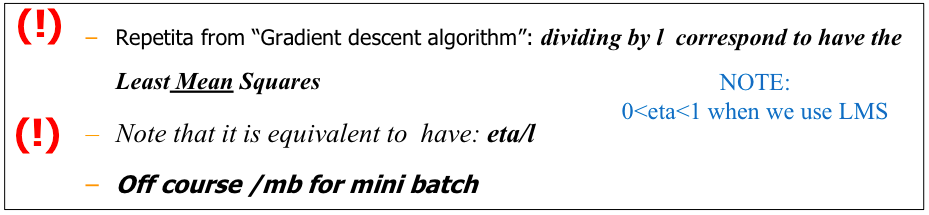
\includegraphics[scale = 0.34]{lectures/4_neural_networks/4_eta_hints.png}
        \label{fig:4_eta_hints}
    \end{figure}
    \begin{itemize}
        \item Take care that on-line can be more unstable!
        \item Note that if you use the “mean” of gradient for the epochs (batch), using on-line training will require much smaller eta to be comparable!!!! (or on the other way an higher eta for the batch case).
    \end{itemize}
    
\end{itemize}

\noindent \textbf{Learning rate and mini batch}\\
Using mini-batch the gradient does not decrease to zero close to a minimum (as the exact gradient can do), hence fixed learning rate should be avoided.\\
For instance \emph{decay linearly} eta for each step until iteration $\tau$, using $\alpha = (step\,\, s)/\tau$, then stop and use fix (small) $\eta$:
$$\eta_s = (1-\alpha)\eta_0 + \alpha \eta_\tau$$
When using the linear schedule, the parameters to choose are $\eta_0$, $\eta_\tau$, and $\tau$. Usually $\tau$ may be set to the number of iterations required to make a few hundred passes through the training set. Usually $\eta_\tau$ should be set to roughly 1 percent the value of $\eta_0$. The main question is how to set $\eta_0$. If it is too large, the learning curve will show violent oscillations, with the cost function often increasing significantly. Gentle oscillations are fine, especially if training with a stochastic cost function, such as the cost function arising from the use of dropout. If the learning rate is too low, learning proceeds slowly, and if the initial learning rate is too low, learning may become stuck with a high cost value.

Typically, the optimal initial learning rate, in terms of total training time and the final cost value, is higher than the learning rate that yields the best performance after the first $100$ iterations or so. Therefore, it is usually best to monitor the first several iterations and use a learning rate that is higher than the best-performing learning rate at this time, but not so high that it causes severe instability. (preliminary trials or grid-search).\\

\newpage
\noindent \textbf{Adaptive Learning Rates}
\begin{itemize}
    \item Use separate eta for each parameter
    \item Automatically adapt during training
    \item Possibly avoiding/reducing the fine tuning phase via hyperparametrs selection
\end{itemize}
E.g.
\begin{itemize}
    \item AdaGrad
    \item RMSProp (becoming quite popular for DL, e.g. caffe SW)
    \item Adam (also popular, often robust with the default value)
    \item ... continuously evolving
\end{itemize}
Combined with moment etc. Popular for DL: see DL book 8.5 if interested.

\subsubsection{Momentum}
$\bigstar$ Backpropagation + Momentum\\

\noindent Remember that the \emph{movements} will be made iteratively according to
$$\bold{w}_{new} = \bold{w}_{old} + \eta \cdot \Delta \bold{w}$$
That can be rewritten as
$$\bold{w}_{new} = \bold{w}_{old} + \Delta \bold{w}_{new}$$
where
\begin{itemize}
    \item \textbf{Without momentum}
    $$\Delta w_{new}=-\eta\frac{\partial E(\bold{w})}{\partial w}$$
    \item \textbf{With momentum}
    $$\Delta w_{new}=-\eta \frac{\partial E(\bold{w})}{\partial w} + \alpha \Delta w_{old}$$
    After you can save $\Delta w_{new}$ for the next step ($\Delta w_{old} = \Delta w_{new})$.
\end{itemize}
\noindent\emph{Momentum parameter} $\alpha$ s.t. $0 < \alpha < 1$ , e.g 0.5 - 0.9

\begin{figure}[H]
    \centering
    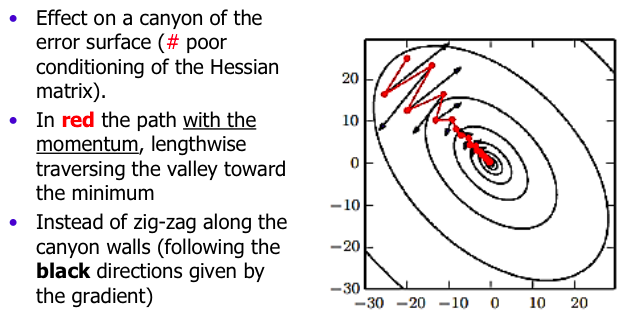
\includegraphics[scale = 0.50]{lectures/4_neural_networks/4_momentum_plot.png}
    \label{fig:4_momentum_plot}
\end{figure}
\begin{itemize}
    \item Faster in plateaus: same sign of gradient for consecutive iterations $\rightarrow$ momentum increases the delta
    \item Damps oscillations: stabilizing effect in directions that oscillate in sign
    \item \emph{Inertia effect}: Allow us to use higher $\eta$ ($0.2 - 0.9$)
    \item Momentum born with \textbf{batch} learning, and it is commonly assumed that helps more in batch mode
    \item In the \textbf{on-line} version can be used resorting to a moving average of the past gradients concept to smooth out the stochastic gradient samples
    
    [e.g. see it in the form grad= alfa grad +(1-alfa) grad\_now ]
    \begin{itemize}
        \item It smooths the gradient over different examples (a different meaning w.r.t. the batch version that uses the same batch of examples)
        \item You can use it multiplying by eta (as usual) for the DeltatW
        \item See if really needed (as any other heuristic)
    \end{itemize}
    
    \item For \textbf{Minibatch}: moving average of past gradients over the progressive minibatchs (that have different examples, not the step before for the same examples as for batch).
\end{itemize}

\noindent $\blacksquare$ \textbf{Nesterov Momentum}\\
Evaluate the gradient after the momentum is applied
\begin{itemize}
    \item First apply the momentum ($\underline{\bold{w}} = \bold{w}_{old} + \alpha \Delta \bold{w}_{old}$)
    \item Evaluate the \emph{new gradient} on this interim point (with such $\underline{\bold{w}}$)
    \item Compute and apply the DeltaW as before (summing the momentum and the \emph{new gradient})
\end{itemize}

So, the new delta rule is:
$$\underline{\bold{w}} = \bold{w}_{old} + \alpha \Delta \bold{w}_{old}$$
$$\Delta w_{new}=-\eta \frac{\partial E(\underline{\bold{w}})}{\partial w} + \alpha \Delta w_{old}$$

$$\bold{w}_{new} = \bold{w}_{old} + \Delta \bold{w}_{new}$$

\begin{figure}[H]
    \centering
    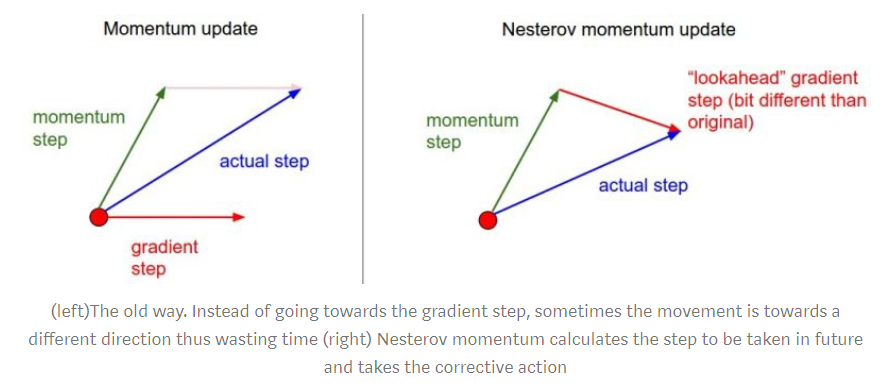
\includegraphics[scale = 0.6]{lectures/4_neural_networks/4_momentums.png}
    \label{fig:4_momentums}
\end{figure}
Shown to improve the rate of convergence for the batch mode (not for the stochastic case!). Popular in SW libraries such is Caffe (DL software)

\subsubsection{optimizers}
\begin{figure}[H]
    \centering
    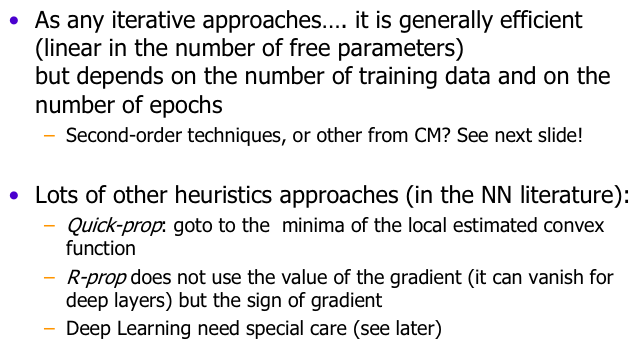
\includegraphics[scale = 0.40]{lectures/4_neural_networks/4_optimizers_1.png}
\end{figure}
\begin{figure}[H]
    \centering
    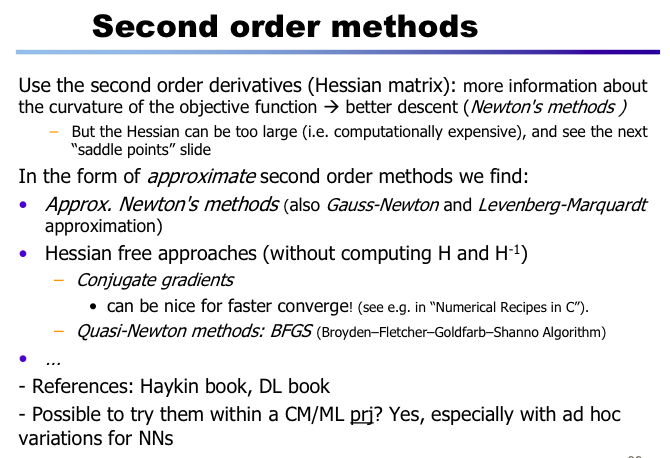
\includegraphics[scale = 0.40]{lectures/4_neural_networks/4_optimizers_2.png}
\end{figure}
\begin{figure}[H]
    \centering
    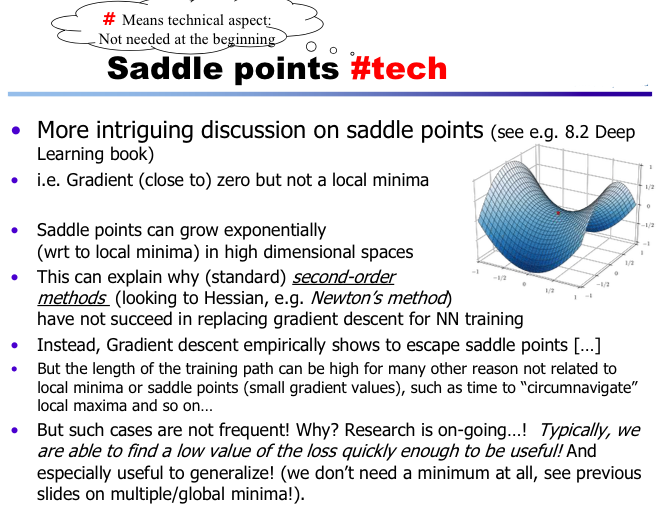
\includegraphics[scale = 0.40]{lectures/4_neural_networks/4_optimizers_3.png}
\end{figure}
\begin{figure}[H]
    \centering
    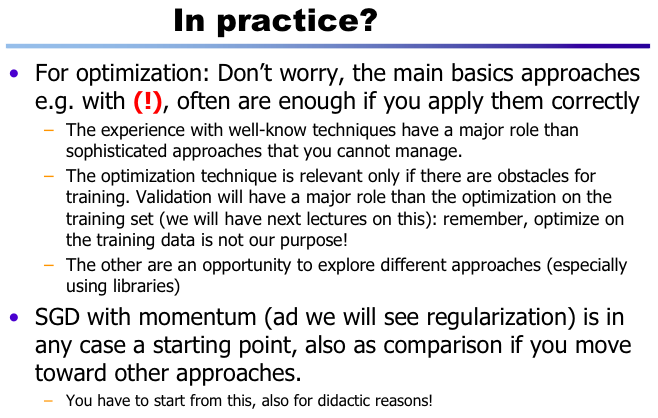
\includegraphics[scale = 0.36]{lectures/4_neural_networks/4_optimizers_4.png}
\end{figure}

\subsubsection{Stopping criteria}
There are many approaches:
\begin{itemize}
    \item The basic is the used loss ($loss<k$); the best if you know the \textbf{tolerance of data (expert knowledge)}.
    \item Max (instead of mean) tolerance on data.
    \item Classification: Number of misclassified (error rate).
    \item No more relevant weight changes/ near zero gradient (Euclidian norm of gradient $< \epsilon$). No more significant error decreasing for a epoch (e.g. less than $0.1\%$).\\
    NOTE: may be premature (e.g. if eta is too small)! It can be applied observing k epochs.
    \item $\bigstar$ In any case stop after an excessive number of epochs.
    \item Not necessarily stop with very low training error...we may be in overfitting (see next). We want a model that is able to generalize the data, so we have to do Validation!
\end{itemize}
\subsubsection{Overfitting and regularization}
$\blacksquare$\textbf{Stopping at the minimum?}\\
\noindent Typically we don’t want the global minimizer of $R_{emp}(w)$, as this is likely to be an overfitting solution (difference with respect to optimization (CM) methods).\\

\noindent The control of complexity it is our main aim to achieve the best generalization capability.\\
For instance we need to add some \emph{regularization}:
\begin{itemize}
    \item this is achieved directly through a \emph{penalty term}, or indirectly by \emph{early stopping}.
    \item Plus model selection (cross-validation) on empirical data to find the trade-off.
\end{itemize}

\noindent$\blacksquare$\textbf{Overfitting in NN}\\
\noindent A neural network that is designed to generalize well will produce a correct
input–output mapping even when the input is slightly different from the examples used
to train the network, as illustrated in the figure. When, however, a neural network learns too many input–output examples, the network may end up memorizing the training
data. It may do so by finding a feature (due to noise, for example) that is present in the training data, but not true of the underlying function that is to be modeled. Such a phenomenon is referred to as \textbf{overfitting} or \textbf{overtraining}. When the network is overtrained, it loses the ability to generalize between similar input–output patterns.\\

\begin{itemize}
    \item Start learning with small weights (symmetry breaking).
    \item The mapping input-output is nearly linear:
    \begin{itemize}
        \item number of effective free parameters (and VC-dim) nearly as in perceptron
    \end{itemize}
    \item As optimization proceeds hidden units tend to \emph{saturate}, \emph{increasing the effective number of free parameters} (and introduce non-linearities) and hence \emph{increase VC-dim}.
    \item A variable-size hypothesis space.
\end{itemize}
\begin{figure}[H]
    \centering
    \includegraphics[scale = 0.35]{lectures/4_neural_networks/4_bp_learning_curve.png}
    \caption{Typical behavior of backprop learning curve}
    \label{fig:4_learning_curve_bp}
\end{figure}
\emph{So, how we can avoid the overfitting?}\\

\noindent$\blacksquare$\textbf{Learning curve analysis}\\
Recall the VC-bound plot! (theoretical ground). This is the learning curve plot for training and validation, same thing with different name. How to act?
\begin{itemize}
    \item \emph{Early stopping}: use a \textbf{validation set} for determining when to stop (at the validation error increasing ... quite vague!)
    \begin{itemize}
        \item Use more than one epoch before estimating (patience).
        \item Backtracking approaches.
        \item Note that since effective number of parameters grows during the course of training, halting training correspond to \emph{limit the effective complexity}.
    \end{itemize}
    \item \emph{Regularization} (on the loss : our main warhorse!)
    \item \emph{Pruning methods} (see later)
\end{itemize}
$\bigstar$\textbf{Regularization}\\
\noindent Training $\rightarrow$ weight increases: we can optimize the loss considering the weight values.\\
A well know principled approach (related to \textbf{Tikhonov theory}):
\begin{figure}[H]
    \centering
    \includegraphics[scale = 0.4]{lectures/4_neural_networks/4_penalty_term.png}
    \label{fig:4_penalty_term}
\end{figure}
\noindent Often we simplified calling equivalently (mean) Loss or Error or Risk the objective function. When we have regularization, as in the Tikhonov regularization, a penalty term in the objective function is better to clarify:
\begin{itemize}
    \item We can use \textbf{Loss} name for the objective function ($MSE+Penalty$) \emph{for model training}.
    \item And \textbf{Error}/Risk for the “data term” (the (M)SE, depending on data)
    $$\sum_{p}(d_p-o(\bold{x}_p))^2$$
    \emph{to evaluate model error}, because this is the measure useful to the user (using the model), and to be reported in the table or plots etc. ($\bigstar$).
\end{itemize}
$\blacksquare$\textbf{Regularization: details}
\begin{itemize}
    \item Note that often the bias $w_0$ is omitted from the regularizer (because its inclusion causes the results to be not independent from target shift/scaling) or it may be included but with its own regularization coefficient (see Bishop book, Hastie et al. book).
    \item Typically apply it in the batch version.
    \item For on-line/mini-batch take care of possible effects over many steps (patterns/examples): hence to compare with respect to batch version in a fair way do not force equal lambda but it would be better to use
    $$\lambda \times mb \over{l}$$
    where $l$ is the number of total patterns.
    \begin{itemize}
        \item Of course if you choose lambda by model selection they will automatically select different lambda for on-line and batch (or any mini-batch)
    \end{itemize}
    \item Other techniques: \textbf{Dropout} (see later).
\end{itemize}
Remember, regularization is for the control of the VC-dim, it has no relation with stability to the error of learning rate of the model.\\
So Regularization vs Learning Curve for the stopping criteria. Learning Curve is an empirical approach instead the regularization approach is not, the learning curve for validation will follow the learning curve for the training, we can stop with some epsilon.\\

$\blacksquare$\textbf{Effect of regularization}
\begin{figure}[H]
    \centering
    \includegraphics[scale = 0.7]{lectures/4_neural_networks/4_reg_effects.png}
    \label{fig:4_reg_effects}
\end{figure}

\noindent $\blacksquare$\textbf{Merging Weight decay + Momentum}
\begin{figure}[H]
    \centering
    \includegraphics[scale = 0.4]{lectures/4_neural_networks/4_mom_reg.png}
    \label{fig:4_mom_reg}
\end{figure}
\subsubsection{Number of hidden units}
\begin{itemize}
    \item Related to the \textbf{control of complexity} issue,
    \item The number can be high if appropriate regularization is used.
    \item Related also to the input dimension and to the size of the TR data set.
\end{itemize}
In general, is a \textbf{model selection} issue:
\begin{itemize}
    \item To few hidden units $\rightarrow$ underfitting
    \item To many hidden units $\rightarrow$ overfitting (can occur)
\end{itemize}
For example by cross-validation on a TR set (part for training) with validation set to select the model (number of units) + external test set to evaluate:
\begin{itemize}
    \item Of course retrain the model for each different configuration!
\end{itemize}
There are two approaches:
\begin{itemize}
    \item \textbf{Constructive approaches}: the learning algorithm decide the number starting with small network and then adding new units.
    \item \textbf{Pruning methods}: start with large networks and progressivelly elimnate weights or units.
\end{itemize}
$\blacksquare$\textbf{Constructive approaches}\\
\noindent Incremental approach: algorithms that build a network starting with a minimal configuration and adds new units and connections during training.\\
Examples:
\begin{itemize}
    \item For classification: Tower, Tiling, Upstart
    \item For both regression and classification: Cascade Correlation
\end{itemize}
An exemplificative and effective approach : the \textbf{Cascade Correlation} learning algorithm:
\begin{itemize}
    \item Start with a minimum networks.
    \item Add units if they are needed until the error is low.
\end{itemize}
It learn both the network weights and network topology (number of units).
\begin{itemize}
    \item automatic determination of network dimension and topology: CC allows to deal with hypothesis spaces of flexible size, since the number of hidden units is decided by the learning algorithm;
    \item training of a single unit for each step.
\end{itemize}
See Scott E. Fahlman and Christian Lebiere:
The Cascade-Correlation Learning Architecture 1991 CMU-CS-90-
100 Carnegie Mellon University Also in NIPS 2, 1990, pages 524-532
\newpage
\textbf{The CC algorithm}
\begin{figure}[H]
    \centering
    \includegraphics[scale = 0.74]{lectures/4_neural_networks/4_cc_alg.png}
    \label{fig:4_cc_alg}
\end{figure}
\begin{figure}[H]
    \centering
    \includegraphics[scale = 0.74]{lectures/4_neural_networks/4_cc_ex.png}
    \label{fig:4_cc_ex}
\end{figure}
\begin{figure}[H]
    \centering
    \includegraphics[scale = 0.74]{lectures/4_neural_networks/4_cc_learn.png}
    \label{fig:4_cc_learn}
\end{figure}

\noindent\textbf{CC Maximization of the correlation}\\
$$ S = \sum_{k}^{n} \left| \sum_{p}^{l} (O_p - mean_p(O))(E_{k,p} - mean_p(E_k)) \right|$$

In order to maximize S, we must compute $\frac{\delta S}{\delta w_j}$, the partial derivative of S with respect to each of the candidate unit's incoming weights, Wi. In a manner very similar to the derivation of the back-propagation rule in [Rumelhart, 1986], we can expand and differentiate the fonnula for S to get:

$$ \frac{\delta S}{\delta w_j} = \sum_{k}^{n} sgn(S_k) \sum_{p}^{l} (E_{k,p} - mean_p(E_k))f'(net_{h,p})I_{j,p} $$
\textit{Derivation:}\\

$$ = \frac{\delta S}{\delta w_j} = \frac{\delta\sum_{k}^{n} \left| \sum_{p}^{l} (O_p - mean_p(O))(E_{k,p} - mean_p(E_k)) \right|}{\delta w_j} = $$

$$\sum_{k}^{n} sgn(S_k) \frac{ \sum_{p}^{l} \delta [(O_p - mean_p(O))(E_{k,p} - mean_p(E_k))]}{\delta w_j}$$

the internal component of $\sum_{p}^{l}$ can be rewritten as:

$$ \frac{\delta [(O_p - mean_p(O))(E_{k,p} - mean_p(E_k))]}{\delta w_j} = (E_{k,p} - mean_p(E_k)) \frac{\delta (O_p - mean_p(O))}{\delta net_p}\frac{\delta net_p}{\delta w_j}=$$
$$ = (E_{k,p} - mean_p(E_k)) \frac{\delta (O_p - mean_p(O))}{\delta O_p}\frac{\delta O_p}{\delta net_p}\frac{\delta net_p}{\delta w_j}$$

we know that the average $mean_p(O)$ is independent of p so:

$$ \frac{\delta (O_p - mean_p(O))}{\delta O_p} = 1 \;, \; \frac{\delta O_p}{\delta net_p} = f'(net_{h,p}) \;\; \text{(where $h$ is the candidate index)} $$

and we can  rewrite:
$$ \frac{\delta net_p}{\delta w_j} = I_{j,p} \;\; \text{input candidate from unit j and pattern p}$$

by bringing it all together we found the solution:

$$ \frac{\delta S}{\delta w_j} = \sum_{k}^{n} sgn(S_k) \sum_{p}^{l} (E_{k,p} - mean_p(E_k))f'(net_{h,p})I_{j,p} $$

Of course, the delta is positive in this case (compared to the case of minimizing the error with backprogration) so we are doing gradient ascent (gradient descent is for the minimization).\\


\textbf{Notes on CC}
\begin{itemize}
    \item The role of hidden units is to reduce the residual output error
    \begin{itemize}
        \item It solve a specific sub-problem
        \item It became a permanent “feature-detector”
    \end{itemize}
    \item POOL: Typically, since the maximization of the correlation is obtained using a gradient ascent technique on a surface with several maxima, a pool of hidden units is trained and the best one selected. This help avoid local maxima.
    \item Greedy algorithms: easy to obtain converge, may also find a minimal number of units but it may lead into overfitting (need regularization).
\end{itemize}
Loss: Not necessarily “max S”: e.g.,for regression, LMS in Prechelet 1997, Neural Networks Vol. 10 pp. 885-896
\subsubsection{Input scaling / Output representation}
$\blacksquare$\textbf{Input}\\
\noindent Preprocessing can have large effect.\\
For different scale values, normalization via :
\begin{itemize}
    \item \emph{Standardizations} (often useful):\\
    For each feature we obtain zero mean and standard deviation 1: $v-mean /standard\,\, dev$.
    \item \emph{Rescaling}: [0,1] range; $v-min /(max-min)$
\end{itemize}
Remember that
\begin{itemize}
    \item \emph{Categorical inputs}:\\
    A $\rightarrow$ 100, B $\rightarrow$ 010, C $\rightarrow$ 001
    \item \emph{Missing data}: 0 does not mean “no input” if 0 is in the input range!
\end{itemize} 
$\blacksquare$\textbf{Output}\\
\noindent\textbf{Classification}\\
\noindent 1-of-K with multioutput
\begin{itemize}
    \item Sigmoid $\rightarrow$ choose the threshold to assign the class.
    \item Rejection zone.
    \item 1-of-K: the highest value
    \begin{itemize}
        \item Often symmetric logistic learn faster (see Haykin)
    \end{itemize}
    \item 0.9 can be used instead of 1 (as d value) to avoid asymptotical convergence (-0.9 for –1 or 0.1 for 0)
\end{itemize}
Of course, target range must be in the output range of units.\\

\noindent\textbf{Regression}\\
\noindent Output \textbf{linear} unit(s).
\begin{figure}[H]
    \centering
    \includegraphics[scale = 0.35]{lectures/4_neural_networks/4_in_out.png}
    \label{fig:4_in_out}
\end{figure}

Open questions:
\begin{itemize}
    \item Reflect on the role of the different hyper-parameters
    \item Connect to the theory (also later after next lectures)
    \begin{itemize}
        \item E.g. relate the optimization of the loss with penalty term to the Statistical Learning Theory (VC-bound in the introduction and next lectures) to understand the role of lambda in controlling under/overfitting cases.
    \end{itemize}
\end{itemize}
Hence, which are the most relevant for your project?
\end{document}

